% Giữ tên và cấu trúc tác giả; số liệu và diễn giải theo bằng chứng hiện hành.
\PassOptionsToPackage{pdfusetitle=false,hypertexnames=false,hidelinks}{hyperref}
\PassOptionsToPackage{hyphens}{url}
\documentclass[preprint,12pt]{elsarticle}

\usepackage[
    left=1.8cm,
    right=1.8cm,
    top=2.0cm,
    bottom=2.0cm
]{geometry}

%% Use the option review to obtain double line spacing
%% \documentclass[authoryear,preprint,review,12pt]{elsarticle}

%% Use the options 1p,twocolumn; 3p; 3p,twocolumn; 5p; or 5p,twocolumn
%% for a journal layout -- left commented, preprint style is used here.
%% \documentclass[final,3p,times]{elsarticle}

%% For including figures, graphicx.sty has been loaded in elsarticle.cls.

%% The amssymb package provides various useful mathematical symbols
\usepackage{amssymb}
%% The amsmath package provides various useful equation environments.
\usepackage{amsmath}

%% Packages required by the original manuscript content (tables,
%% algorithms, float placement) -- preserved from the source document.
\usepackage[T1]{fontenc}
\usepackage{lmodern}
\usepackage[utf8]{inputenc}
\usepackage[english]{babel}
\usepackage{xcolor}
\usepackage{amsmath}
\usepackage{graphicx}
\usepackage{tabularx}
\usepackage{booktabs}
\usepackage{float}
\usepackage[ruled,vlined,linesnumbered]{algorithm2e}
\usepackage[section]{placeins}


\usepackage{orcidlink}
\usepackage{tikz}
\usetikzlibrary{arrows.meta}
\usepackage{hyperref}
% Kiểu trình bày chung; không thay giá trị thực nghiệm hoặc metadata tác giả.
\hypersetup{pdftitle={Evaluating Quantitative Alpha and News Sentiment in QuantAgent for Vietnamese Stock Trading}}
% Ưu tiên ghép bảng/hình với văn bản, giữ khoảng cách vừa đủ và tránh giãn dọc trang.
\raggedbottom
\renewcommand{\topfraction}{0.95}
\renewcommand{\bottomfraction}{0.95}
\renewcommand{\textfraction}{0.05}
\renewcommand{\floatpagefraction}{0.8}
\setcounter{topnumber}{4}
\setcounter{bottomnumber}{4}
\setcounter{totalnumber}{6}
\setlength{\floatsep}{10pt plus 2pt minus 2pt}
\setlength{\textfloatsep}{12pt plus 2pt minus 3pt}
\setlength{\intextsep}{10pt plus 2pt minus 2pt}
% Footer trung tính, không suy rằng bản thảo đã được gửi tới tạp chí.
\date{12 November 2026}
\makeatletter
% Căn đầu trang float; không kéo giãn khoảng cách giữa các bảng trên cùng trang.
\setlength{\@fptop}{0pt}
\setlength{\@fpsep}{12pt plus 2pt minus 2pt}
\setlength{\@fpbot}{0pt plus 1fil}
\pdfstringdefDisableCommands{\let\orcidlink\@gobble\let\corref\@gobble\def\,{ }\let\cnotenum\@empty\let\@corref\@empty}
\def\ps@pprintTitle{%
  \let\@oddhead\@empty
  \let\@evenhead\@empty
  \def\@oddfoot{\footnotesize\itshape Research manuscript\hfill\@date}%
  \let\@evenfoot\@oddfoot}
\makeatother


\journal{Knowledge-Based Systems}

%% Figures live under figures/figs/... in this project; original
%% \includegraphics calls use the relative path "figs/..." as in the
%% source manuscript, so we add "figures/" to the graphics search path.
\graphicspath{{./}}

\newcommand{\FullBA}{52.96}
\newcommand{\BaseBA}{49.71}
\newcommand{\FullAccuracy}{65.69}
\newcommand{\BaseAccuracy}{60.78}
\newcommand{\CashAccuracy}{75.49}
\newcommand{\LogisticPriceBA}{55.61}
\newcommand{\FullReturn}{-0.797}
\newcommand{\BaseReturn}{-0.750}
\newcommand{\DeltaBA}{3.25}
\newcommand{\PrimaryLow}{-1.18}
\newcommand{\PrimaryHigh}{8.13}

\newcommand{\UnifiedPoints}{102}
\newcommand{\UnifiedAccounts}{51}
\newcommand{\UnifiedSymbols}{9}
\newcommand{\UnifiedDates}{12}
\newcommand{\UnifiedFolds}{6}
\newcommand{\UnifiedMissingSentiment}{79}
\newcommand{\UnifiedUpstreamRealizations}{1}
\newcommand{\UnifiedDecisionRepeats}{3}
\newcommand{\UnifiedForecastSlots}{2448}
\newcommand{\UnifiedNativeReturn}{-0.653}
\newcommand{\UnifiedNativeBA}{51.84}
\newcommand{\UnifiedNativeRaw}{306}
\newcommand{\UnifiedNativeBypass}{0}
\newcommand{\UnifiedCommonReturn}{-1.025}
\newcommand{\UnifiedCommonBA}{45.97}
\newcommand{\UnifiedCommonRaw}{306}
\newcommand{\UnifiedCommonBypass}{0}
\newcommand{\UnifiedVOneReturn}{-0.698}
\newcommand{\UnifiedVOneBA}{50.10}
\newcommand{\UnifiedVOneRaw}{144}
\newcommand{\UnifiedVOneBypass}{162}
\newcommand{\UnifiedCTwoReturn}{-1.030}
\newcommand{\UnifiedCTwoBA}{45.75}
\newcommand{\UnifiedCTwoRaw}{3}
\newcommand{\UnifiedCTwoBypass}{303}
\newcommand{\UnifiedAPoolReturn}{-1.019}
\newcommand{\UnifiedAPoolBA}{46.18}
\newcommand{\UnifiedAPoolRaw}{24}
\newcommand{\UnifiedAPoolBypass}{282}
\newcommand{\UnifiedBSemanticReturn}{-1.030}
\newcommand{\UnifiedBSemanticBA}{45.75}
\newcommand{\UnifiedBSemanticRaw}{3}
\newcommand{\UnifiedBSemanticBypass}{303}
\newcommand{\UnifiedMTReturn}{-1.253}
\newcommand{\UnifiedMTBA}{43.17}
\newcommand{\UnifiedMTRaw}{198}
\newcommand{\UnifiedMTBypass}{108}
\newcommand{\UnifiedFactAnchorReturn}{-1.286}
\newcommand{\UnifiedFactAnchorBA}{42.74}
\newcommand{\UnifiedFactAnchorRaw}{306}
\newcommand{\UnifiedFactAnchorBypass}{0}
\newcommand{\UnifiedCashReturn}{0.000}
\newcommand{\UnifiedCashBA}{50.00}
\newcommand{\UnifiedCashRaw}{0}
\newcommand{\UnifiedCashBypass}{306}
\newcommand{\UnifiedAlwaysLongReturn}{-3.000}
\newcommand{\UnifiedAlwaysLongBA}{50.00}
\newcommand{\UnifiedAlwaysLongRaw}{0}
\newcommand{\UnifiedAlwaysLongBypass}{306}
\newcommand{\UnifiedVOneNativeReturnEffect}{-0.045}
\newcommand{\UnifiedVOneNativeReturnLow}{-0.362}
\newcommand{\UnifiedVOneNativeReturnHigh}{0.271}
\newcommand{\UnifiedCTwoNativeReturnEffect}{-0.377}
\newcommand{\UnifiedCTwoNativeReturnLow}{-0.866}
\newcommand{\UnifiedCTwoNativeReturnHigh}{0.111}
\newcommand{\UnifiedAPoolNativeReturnEffect}{-0.367}
\newcommand{\UnifiedAPoolNativeReturnLow}{-0.867}
\newcommand{\UnifiedAPoolNativeReturnHigh}{0.133}
\newcommand{\UnifiedBSemanticNativeReturnEffect}{-0.377}
\newcommand{\UnifiedBSemanticNativeReturnLow}{-0.866}
\newcommand{\UnifiedBSemanticNativeReturnHigh}{0.111}
\newcommand{\UnifiedMTNativeReturnEffect}{-0.601}
\newcommand{\UnifiedMTNativeReturnLow}{-1.090}
\newcommand{\UnifiedMTNativeReturnHigh}{-0.111}
\newcommand{\UnifiedVOneCommonReturnEffect}{0.327}
\newcommand{\UnifiedVOneCommonReturnLow}{0.067}
\newcommand{\UnifiedVOneCommonReturnHigh}{0.586}
\newcommand{\UnifiedCTwoCommonReturnEffect}{-0.005}
\newcommand{\UnifiedCTwoCommonReturnLow}{-0.016}
\newcommand{\UnifiedCTwoCommonReturnHigh}{0.005}
\newcommand{\UnifiedAPoolCommonReturnEffect}{0.005}
\newcommand{\UnifiedAPoolCommonReturnLow}{-0.005}
\newcommand{\UnifiedAPoolCommonReturnHigh}{0.016}
\newcommand{\UnifiedBSemanticCommonReturnEffect}{-0.005}
\newcommand{\UnifiedBSemanticCommonReturnLow}{-0.016}
\newcommand{\UnifiedBSemanticCommonReturnHigh}{0.005}
\newcommand{\UnifiedMTCommonReturnEffect}{-0.229}
\newcommand{\UnifiedMTCommonReturnLow}{-0.576}
\newcommand{\UnifiedMTCommonReturnHigh}{0.118}
\newcommand{\UnifiedVOneNativeBAEffect}{-1.749}
\newcommand{\UnifiedVOneNativeBALow}{-6.374}
\newcommand{\UnifiedVOneNativeBAHigh}{2.876}
\newcommand{\UnifiedCTwoNativeBAEffect}{-6.095}
\newcommand{\UnifiedCTwoNativeBALow}{-11.629}
\newcommand{\UnifiedCTwoNativeBAHigh}{-0.561}
\newcommand{\UnifiedAPoolNativeBAEffect}{-5.662}
\newcommand{\UnifiedAPoolNativeBALow}{-11.771}
\newcommand{\UnifiedAPoolNativeBAHigh}{0.446}
\newcommand{\UnifiedBSemanticNativeBAEffect}{-6.095}
\newcommand{\UnifiedBSemanticNativeBALow}{-11.629}
\newcommand{\UnifiedBSemanticNativeBAHigh}{-0.561}
\newcommand{\UnifiedMTNativeBAEffect}{-8.675}
\newcommand{\UnifiedMTNativeBALow}{-20.239}
\newcommand{\UnifiedMTNativeBAHigh}{2.888}
\newcommand{\UnifiedVOneCommonBAEffect}{4.130}
\newcommand{\UnifiedVOneCommonBALow}{2.011}
\newcommand{\UnifiedVOneCommonBAHigh}{6.249}
\newcommand{\UnifiedCTwoCommonBAEffect}{-0.216}
\newcommand{\UnifiedCTwoCommonBALow}{-0.668}
\newcommand{\UnifiedCTwoCommonBAHigh}{0.235}
\newcommand{\UnifiedAPoolCommonBAEffect}{0.216}
\newcommand{\UnifiedAPoolCommonBALow}{-0.235}
\newcommand{\UnifiedAPoolCommonBAHigh}{0.668}
\newcommand{\UnifiedBSemanticCommonBAEffect}{-0.216}
\newcommand{\UnifiedBSemanticCommonBALow}{-0.668}
\newcommand{\UnifiedBSemanticCommonBAHigh}{0.235}
\newcommand{\UnifiedMTCommonBAEffect}{-2.797}
\newcommand{\UnifiedMTCommonBALow}{-11.168}
\newcommand{\UnifiedMTCommonBAHigh}{5.575}


\begin{document}

\begin{frontmatter}

%% Title, authors and addresses

\title{Enhancing Multi-Agent Large Language Models for Stock Trading through Quantitative Alpha Integration\tnoteref{t1}}
\tnotetext[t1]{This research is funded by Foreign Trade University under research program number FTURP02-2026-08.}

%% Authors
\author[1]{Hong-Viet Tran\,\orcidlink{0000-0002-4675-2123}}
\author[1]{Hoang-Dung Phan\,\orcidlink{0009-0003-6859-0852}}
\author[1,2]{Thanh-Tam Do Thi\,\orcidlink{0000-0002-7594-276X}}
\author[1]{Phuong-Thai Nguyen\,\orcidlink{0009-0006-2033-7788}}
\author[3]{Van-Tang Nguyen\,\corref{cor1}\orcidlink{0009-0009-7266-2437}}

%% Affiliations
\affiliation[1]{organization={Institute for Artificial Intelligence, University of Engineering and Technology, Vietnam National University},
            city={Hanoi},
            country={Vietnam}}

\affiliation[2]{organization={Faculty of Economic Information System and E-Commerce, Thuongmai University},
            city={Hanoi},
            country={Vietnam}}

\affiliation[3]{organization={Faculty of Technology and Data Science, Foreign Trade University},
            city={Hanoi},
            country={Vietnam}}

\cortext[cor1]{Corresponding author}


%% Abstract
\begin{abstract}
We propose a method for integrating chart, price--volume and news
evidence in a multi-agent large language model (LLM) system for daily
Vietnamese equity trading. Vision--language agents interpret chart
patterns and trends. A deterministic Alpha Agent ranks 85 candidate
price--volume factors and summarizes selected signals as a direction
and vote counts. A Sentiment Agent uses a ViSoBERT-based classifier to
score eligible Vietnamese-language news and flags insufficient coverage.
The LLM Decision Agent combines these structured summaries with the
technical reports in a single prompt to make a directional forecast
for a long-or-cash strategy.
We compare the augmented system with the price-only QuantAgent baseline
at 102 paired stock--date cutoffs. Both systems receive the same
technical reports and use the same T+2.5 execution and trading costs.
A prompt audit verifies which signals reach the decision model.
In this historical sample, both systems identified seven profitable
LONG opportunities. False LONG calls decreased from 22 to 17, and
balanced accuracy rose from 49.71\% to 52.96\%. Mean net account return
was slightly lower for the augmented system, and limited news coverage
constrains attribution to sentiment. A separate study evaluates five
Bayesian in-context learning variants that condition decisions on
completed trading episodes.
\end{abstract}

%%Graphical abstract


\begin{highlights}
\item A multi-agent LLM system fuses chart, price--volume and news evidence.
\item Alpha votes and Vietnamese news sentiment inform the LLM decision prompt.
\item Shared technical reports support paired tests at 102 stock--date cutoffs.
\item The system cut false LONG calls from 22 to 17 and retained 7 true positives.
\item Five Bayesian in-context variants use completed trading episodes.
\end{highlights}

%% Keywords
\begin{keyword}
Multi-agent LLM \sep Knowledge fusion \sep Knowledge integration \sep Financial decision support \sep Alpha factor selection
\end{keyword}

\end{frontmatter}


%% main text
\section{Introduction}
\label{sec:introduction}

QuantAgent \cite{xiong2025quantagent} decomposes price-driven trading into roles for technical indicators, chart patterns, trends and risk. This paper asks whether adding quantitative alpha and Vietnamese news sentiment makes that architecture more effective for daily Vietnamese-equity forecasts. We call the augmented configuration \emph{Our system}. We test it against a local price-only implementation of the QuantAgent architecture under the same daily trading protocol. The original publication studies a different market setting and trading horizon.

We integrate an OHLCV alpha selector and Vietnamese sentiment with Indicator, Pattern, Trend and Decision roles adapted from QuantAgent. The selector ranks 85 candidate factors, while sentiment enters a separate textual report. Numerical indicators, chart descriptions and the enabled factor/news reports are condensed into the Decision prompt with heuristic evidence priorities. The resulting binary forecast is evaluated against a net three-session LONG cycle; a bearish forecast maps to CASH in the long-only account.

The primary component study compares Our system and QuantAgent on 102 paired stock--date observations across nine equities, twelve dates and six historical blocks. Small repeated panels examine upstream variability, alpha-only and sentiment-only variants, and a matched-structure placebo. BICL v1--v5 form a secondary extension study asking what historical context adds once the alpha and sentiment channels are already present. The historical evaluation and its repaired rerun each use three Decision repeats with one shared upstream realization per point. We report those collections separately.

In the component study, Our system reaches \FullBA\% balanced accuracy (BA), versus \BaseBA\% for QuantAgent and \LogisticPriceBA\% for a price-only logistic comparator. Both agent systems identify seven of the 25 UP outcomes. Our system makes fewer false LONG forecasts, giving a \DeltaBA{} percentage-point BA advantage, while its mean separate-account net return is slightly lower. The paired result supports a limited improvement in classification. The small component panels and the historical coverage of news leave the separate effects of alpha and sentiment uncertain.

The contributions are:
\begin{itemize}
\item A Vietnamese-equity implementation that combines an 85-candidate OHLCV selector and local-language sentiment with shared chart-agent reports.
\item A paired comparison with QuantAgent that measures class-aware forecasts, distinguishable component interventions and transaction-cost-aware account outcomes.
\item Five BICL extensions evaluated against augmented-system controls, with explicit historical support, fallback and action-revision rules.
\end{itemize}

The analysis is historical and exploratory: the evaluation schedule was finalized after some inference, market outcomes precede the November 2026 data freeze, and only twelve dates are represented. Our system within-history noncausality, uncertain historical news availability and limited repetitions constrain causal and deployment conclusions. These limitations motivate interpreting the system as a documented decision-support experiment.

The remainder of the paper reviews related work, formalises the forecasting task, describes the agents and experiments, reports results, and discusses limitations and future work.

\section{Related Work}
\label{sec:relatedworks}

\subsection{LLM Agents in Financial Analysis}
TradingAgents~\cite{tradingagents2024} assigns financial analysis, debate,
trading and risk to specialist roles. FinMem~\cite{yu2025finmem} uses
layered memory to organize financial information for a trading agent.
QuantAgent~\cite{xiong2025quantagent} specializes in short-horizon
price-driven signals. Our comparison tests what explicit price--volume
factors and local news add to the same technical reports.

\subsection{Technical Analysis and Pattern Recognition}
Lo et al.~\cite{lo2000technical} formalize chart-pattern recognition and
examine conditional returns. ChartLlama~\cite{han2023chartllama} studies
multimodal chart understanding. They motivate the use of numerical indicators and chart images as
separate inputs.

\subsection{Quantitative Alpha Factor Research}
The \emph{101 Formulaic Alphas} catalogue~\cite{kakushadze2016formulaic}
supplies source expressions. Candidate search raises multiple-testing
concerns~\cite{harvey2016}. We distinguish in-sample diagnostics from
chronological assessment and use Holm's procedure~\cite{holm1979multiple}
for the declared numerical-control family.

\subsection{Sentiment Analysis in Finance and Vietnamese NLP}
Tetlock~\cite{tetlock2007news} relates financial-media tone to market
activity. FinBERT~\cite{araci2019finbert} adapts a language model to
financial sentiment. ViSoBERT~\cite{nguyen2023visobert} is a Vietnamese
social-media backbone. The downstream 5CD-AI classifier~\cite{hf5cdsentiment}
requires separate assessment on Vietnamese financial news.

\subsection{Regime Context and In-Context Learning}
Hidden Markov models~\cite{rabiner1989hmm} distinguish filtering at the
current cutoff from smoothing with later observations. Xie et
al.~\cite{xie2022implicitbayes} study implicit Bayesian inference under a
mixture-of-HMMs construction. Rubin et al.~\cite{rubin2022retrieve} learn
to retrieve in-context examples. These ideas motivate the secondary study of eligible historical episodes and
explicit numerical updates.

\subsection{Evaluation in Emerging Markets}
Local-language news, market calendars and settlement assumptions affect
which information and trades are admissible. A purposive sample supports
comparisons on the observed equities and cutoffs.

\section{Problem Formulation}
\label{sec:formulation}

\subsection{Market Model and Data}
For a given stock, let \(t\) be the last observed session at the decision
cutoff. Indicator and chart tools use the 45 daily open, high, low, close and
volume (OHLCV) bars through \(t\). Alpha uses up to 600 observed bars through
the same cutoff. The 2022 Vietnam Securities Depository schedule~\cite{vsd2022settlement}
allows resale in the afternoon of T+2, counting T from the purchase date.
We use T+2.5 to denote the corresponding daily-bar convention
throughout the evaluation. LONG enters at the next observed Open
\(O_{t+1}\) and exits at the observed Close \(C_{t+3}\) two sessions after
entry. The session index counts observed bars. Calendar and execution
evidence are checked separately, and incomplete cycles have no label.

\subsection{Directional Prediction Task}
The target asks whether a candidate LONG would earn a positive net return.
With fee \(f=0.0025\) and slippage \(s=0.001\) applied on each leg, it is
\begin{equation}
  r_t = \frac{C_{t+3}}{O_{t+1}}
        \frac{(1-s)(1-f)}{(1+s)(1+f)}-1,
  \qquad
  y_t =
  \begin{cases}
    \mathrm{UP},   & r_t>0,\\
    \mathrm{DOWN}, & r_t\leq 0 .
  \end{cases}
  \label{eq:label}
\end{equation}
A LONG prediction maps to a buy followed by liquidation. SHORT maps to
CASH in the long-only ledger. For a complete account with non-overlapping
cycles and fractional execution at the reference prices, let \(a_t=1\)
for LONG and \(a_t=0\) for CASH. Its net return is
\(\prod_t(1+a_t r_t)-1\). Scenarios with lot sizes, delayed fills or pending
cash use their own ledger. The follow-up scores direction only where the
candidate LONG label is defined and compares account returns only where both
scheduled cycles meet the rule, even when a method chose CASH.

\subsection{Alpha Factor Formalisation and Adaptation}
\label{sec:alpha-representation}
The native registry combines 80 adaptations of
\emph{101 Formulaic Alphas}~\cite{kakushadze2016formulaic} with five
custom price--volume factors. A cross-sectional rank becomes a rank
against a stock's own trailing observations (20 bars by default).
Average daily volume uses recorded share volume, and the daily
typical-price proxy substitutes for intraday volume-weighted average price.
These changes alter what the source expressions measure. The registry
excludes 17 industry-neutralisation expressions, one market-capitalisation
expression and three price/volume expressions whose exclusion rationale is
undocumented. The custom formulas are given in \ref{app:signals}.

The native z-score--tanh transformation uses statistics from the supplied
prefix. Some handlers also fill earlier values or choose a volume proxy
from the supplied frame. The prefix ends at the decision cutoff, but its
later rows can still change an earlier diagnostic value. The causal
projection uses row-available operators and expanding normalization.

\subsection{Walk-Forward Alpha Selection}
The native rank uses the absolute Spearman information
coefficient (IC)~\cite{grinold1999active} between a factor and next-entry
net returns. A negative IC reverses the factor for the diagnostics and
report. Directional accuracy uses absolute scores above 0.05 and defaults
to 0.5 with fewer than ten such signals. The ranking Sharpe proxy uses
factor-signed net returns and population standard deviation. The account
ledger uses the actual LONG or CASH action. On the eligible candidate set \(\mathcal V\), let \(\mathcal N\)
be min--max scaling within a metric, with a value of 0.5 on a flat range.
The native score is
\begin{equation}
  S_k=0.40\,\mathcal N_{\mathcal V}(|\mathrm{IC}_k|)
      +0.35\,\mathcal N_{\mathcal V}(\mathrm{Acc}_k)
      +0.25\,\mathcal N_{\mathcal V}(\mathrm{Sharpe}_k).
  \label{eq:composite}
\end{equation}
Up to five candidates are reported after ranking the displayed scores.
Orientation and ranking reuse the same observations, so these are
selection diagnostics. The causal projection fits orientation on training
data and picks five factors and a threshold on purged validation data.
It freezes those choices and preprocessing before the test queries.

The earlier historical-context study paired the native Our system
projection with the common causal projection used by the BICL branches.
The follow-up uses the same causal alpha values for Our system and Common
and retains their distinct Decision prompts.

\subsection{Sentiment Signal Construction}
The Sentiment Agent uses the pinned
5CD-AI Vietnamese sentiment classifier~\cite{hf5cdsentiment}, built on
ViSoBERT~\cite{nguyen2023visobert}. For admitted articles \(i\), it
weights polarity \(\rho_i=P_i(\mathrm{POS})-P_i(\mathrm{NEG})\) by
publication age \(\Delta_i\) in days:
\begin{equation}
  S_t=\frac{\sum_i w_i\rho_i}{\sum_i w_i},
  \qquad w_i=2^{-\Delta_i/30}.
\end{equation}
The 90-day window requires three distinct, dated articles with accepted
scorer provenance and finite scores. Date-only publication is treated as
available the next day. The separate reliability flag requires at least
eight articles. Reported missingness means insufficient eligible evidence.
The historical provider supplies an aggregate and count, so peer-relative
fields on that path are placeholders. The follow-up supplies a missing-context record at each cutoff because
historical news availability could not be verified.

\subsection{Multi-Agent Decision Function}
QuantAgent~\cite{xiong2025quantagent} uses the shared Indicator, Pattern
and Trend reports. Our system adds the Alpha and Sentiment reports.
Component controls retain alpha only (A), sentiment only (S), or current
sentiment with past-donor alpha values (P). The backtest formats the
additional reports without an extra Alpha LLM call. The Decision Agent
receives the variant-specific prompt and emits LONG or SHORT. Historical
context branches can retain a completed parent action when their dependency
or revision rules apply. The scored prediction follows the final action,
and the ledger keeps the raw proposal separately.

BICL v5 estimates the probability of UP from separate historical and
target tasks. A Beta--Bernoulli teacher supplies probability draws
\(\theta\) for the utility check. With net-gain magnitude \(g\) and
loss magnitude \(\ell\),
\begin{equation}
  U(\mathrm{LONG})=\theta g-(1-\theta)\ell,\qquad
  U(\mathrm{CASH})=0,\qquad
  \Delta U=U(a^{\mathrm{proposed}})-U(a^0),
  \label{eq:revision_utility}
\end{equation}
where \(a^0\) is the Fact Anchor action. An eligible, fact-checked
revision replaces the anchor only if \(Q_{0.10}(\Delta U)>0\).
The utility quantile describes the specified teacher and magnitude model.

\subsection{Walk-Forward Evaluation Protocol}
Algorithm~\ref{alg:shared-reports} describes how the price-only and augmented
systems produce paired decisions and how BICL branches add context in the follow-up evaluation.

\begin{algorithm}[H]
\SetKwInOut{AlgInput}{Input}
\SetKwInOut{AlgOutput}{Output}
\caption{Walk-forward decisions with shared technical reports.}
\label{alg:shared-reports}
\AlgInput{Daily OHLCV, alpha registry, dated news, scheduled cutoffs,
          frozen historical resources and paired branch/repeat schedule.}
\AlgOutput{Recorded proposals and final actions, paired metrics and separate accounts.}
Reserve the evaluation cutoffs outside the historical bank\;
\ForEach{stock and decision cutoff \(t\) in chronological order}{
  Bound prices and dated news at \(t\); retrieve only cycles that ended before \(t\)\;
  Run Indicator, Pattern and Trend once for the shared upstream realization\;
  Prepare the profile-specific alpha and sentiment sections\;
  For follow-up retrieval, derive Trend and Pattern keys from cutoff OHLCV\;
  Freeze the reports and chart inputs; give each branch an independent copy\;
  \ForEach{Decision repeat and branch in dependency order}{
    Build the branch prompt from shared technical reports and its enabled evidence\;
    Add the eligible prior or task context for the corresponding BICL branch\;
    \eIf{the branch must reuse a parent action}{
      Record the same-repeat action and the reason for reuse\;
    }{
      Obtain a Decision proposal through retry and checkpoint handling\;
      Resolve the proposal under the branch policy and save the final action\;
    }
  }
}
After forecasts are locked, join eligible outcomes using Eq.~\ref{eq:label}\;
Score paired decisions and update separate LONG/CASH ledgers\;
\KwRet{the forecast records, account ledgers and paired metrics}\;
\end{algorithm}

The scheduled dates are evaluated chronologically with purging at the
train--validation and validation--test boundaries. Paired branches
reuse one upstream snapshot per point within each shared-report panel.
Historical context is frozen before the first query in a fold and excludes
all reserved evaluation points. Each retrieved cycle must have exited
strictly before the decision date. In the follow-up, forecasts are locked
before evaluation outcomes are computed. Section~\ref{sec:experimentalsetup}
gives the schedules, repetitions and account-level comparisons.

\section{System architecture}
\label{sec:systemarchitecture}
\subsection{Overview}
The implementation uses a LangGraph \cite{langgraph_docs} directed graph with five specialised roles and a shared typed state. Indicator, Pattern, Trend and Decision roles, shared state, chart tools and trendline procedures reuse or modify QuantAgent components; the upstream MIT notice is preserved in the repository \cite{xiong2025quantagent}. Alpha adds numerical factor and Vietnamese sentiment reports. This integration is an engineering adaptation, distinct from inventing the inherited graph or validating a learned knowledge-fusion method.

The historical-context study compares eight research methods and two economic controls. Native uses the native alpha report and instructions; Common uses a training-fitted causal alpha projection with a common prompt and both alpha and sentiment enabled. Four historical priors depend on Common. Fact anchor also receives Common's completed decision, and MT-BICL receives both Common and Fact anchor for the same repeat. The component study separately compares Full and Base by switching factor and sentiment sections.

Figure~\ref{fig:flow} shows the shared upstream, native/common projections and extension dependency schedule. In the evaluated backtest, Indicator is deterministic and the numerical/report Alpha path bypasses an additional alpha-reasoning LLM call. Pattern and Trend consume their separate chart images, while Decision receives the condensed reports and enabled quantitative/text sections. The five role names consequently do not imply five hosted LLM calls per forecast. Model aliases and actual request accounting are specified in Section~\ref{sec:experimentalsetup}.

\begin{figure}[htb]
\centering
% Sơ đồ hai nhánh cho so sánh chính, lịch sử nằm ở nhánh mở rộng.
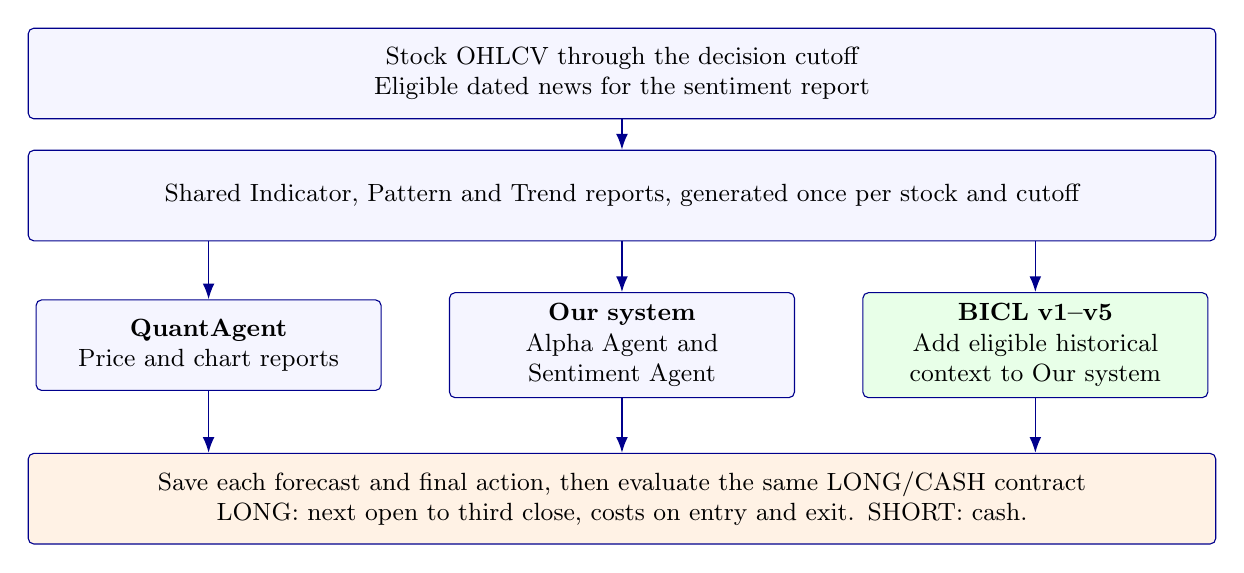
\begin{tikzpicture}[
 box/.style={draw=blue!55!black,rounded corners=2pt,fill=blue!4,align=center,
   text width=4.1cm,minimum height=1.15cm,font=\small,inner sep=4pt},
 wide/.style={box,text width=14.8cm},
 flow/.style={-{Latex[length=2mm]},semithick,draw=blue!55!black}]
\node[wide] (input) at (5.25,0) {Stock OHLCV through the decision cutoff\\Eligible dated news for the sentiment report};
\node[wide] (shared) at (5.25,-1.55) {Shared Indicator, Pattern and Trend reports, generated once per stock and cutoff};
\node[box] (qa) at (0,-3.45) {\textbf{QuantAgent}\\Price and chart reports};
\node[box] (ours) at (5.25,-3.45) {\textbf{Our system}\\Alpha Agent and Sentiment Agent};
\node[box,fill=green!9] (bicl) at (10.5,-3.45) {\textbf{BICL v1--v5}\\Add eligible historical context to Our system};
\node[wide,fill=orange!10] (outcome) at (5.25,-5.4) {Save each forecast and final action, then evaluate the same LONG/CASH contract\\LONG: next open to third close, costs on entry and exit. SHORT: cash.};
\draw[flow] (input)--(shared);
\foreach \step in {qa,ours,bicl}{
  \draw[flow] (\step.north |- shared.south)--(\step.north);
  \draw[flow] (\step.south)--(\step.south |- outcome.north);
}
\end{tikzpicture}

\caption{Shared-report architecture for component and historical-context comparisons.}
\label{fig:flow}
\end{figure}

\subsection{Indicator Agent}
Indicator Agent converts five TA-Lib-based technical indicators into a structured report of bullish, bearish and neutral votes. Table~\ref{tab:indicator_overview} summarises the periods, information and interpretation of each indicator; their technical-analysis foundations follow \cite{appel2005technical,murphy1999technical}. Its backtest node returns a report and messages, without calling an LLM or forwarding the declared state schema's complete numeric arrays. Bollinger variables can be computed on the alpha path; BB/ADX state declarations do not create two additional Indicator votes. \ref{app:indicator_logic} specifies the ordered boundaries and missing-data convention \cite{talib_rsi_docs,talib_willr_docs}.

\begin{table}[htb]
\centering\small
\renewcommand{\arraystretch}{1.18}
\caption{Technical indicators and their roles in the Indicator Agent.}
\label{tab:indicator_overview}
\begin{tabularx}{\textwidth}{p{2.0cm}p{1.6cm}XX}
\hline
Indicator & Periods & Information supplied & Vote interpretation \\
\hline
MACD & 12, 26, 9 & Fast/slow moving-average difference, signal line and histogram. & Crossovers take priority, followed by histogram sign and change. \\
RSI & 14 & Relative strength of recent upward and downward price changes. & Ordered level thresholds and retained-sample direction determine the vote. \\
Stochastic & 14, 3, 3 & Smoothed \%K and \%D locate the close within its recent price range. & Crossovers take priority over overbought/oversold levels and interior rules. \\
Williams \%R & 14 & Position of the close relative to the recent high--low range. & Extreme levels take priority, followed by retained-sample direction. \\
ROC & 10 & Percentage price change over the lookback window. & Values above $+0.5\%$ or below $-0.5\%$ yield bullish or bearish votes. \\
\hline
\end{tabularx}
\end{table}

Four-decimal rounding precedes classification, nonfinite samples are removed and zero is retained. Crossovers take priority where specified; overlapping RSI/Williams thresholds require ordered branches rather than two simultaneous unconditional rules. Each missing/error result contributes a neutral vote within the fixed denominator of five. Directional plurality and the confidence categories are deterministic summary heuristics. They are not calibrated probabilities, and an immutable signal tally does not make a downstream narrative correct.

\subsection{Alpha Agent}
\paragraph{Alpha selection}
The Alpha role evaluates 85 native candidates: 80 retained WorldQuant adaptations and five custom formulas. It supplies a selected top-five report from the trailing prefix, using the diagnostic score in Eq.~\ref{eq:composite}. The transformations, metric support, IC orientation and native row-wise causal failure are defined in Section~\ref{sec:formulation}. A rolling own-history rank is not a cross-sectional rank, and the 21 exclusions are not all justified by an inability to translate cross-sectional operators. Full expressions and exception handling remain in the registry; \ref{app:signals} gives the custom formulas needed to read the reports.

Selection, IC sign and candidate diagnostics reuse trailing observations. Hence the current value is an input to a report, while the reported skill fields are in-sample ranking statistics. Neither choosing the top five nor reversing negative IC establishes out-of-sample profitability. Six selected metadata slots have description/handler mismatches; actual prompts, metadata and implementation identity are kept distinct. The semantic effect of these mismatches is unmeasured.

\paragraph{Common projection and shared parent}
The extension binds a frozen selector to the same point, price prefix and native snapshot hash. Only the alpha report/factor fields are replaced for common-profile consumers; Indicator, Pattern, Trend, chart inputs and sentiment remain shared. Selector fits precede the test scope and are not repeated on a Decision repeat. Native is preserved for comparison rather than silently upgraded. The bridge therefore controls upstream realization while deliberately changing alpha representation and instruction family.

\paragraph{Sentiment integration}
Vietnamese sentiment is a separate contextual report, not an input to the native OHLCV factor formulas or score. The frozen provider supplies aggregate/count information and empty article-detail/peer lists. Relative sentiment and z-score fields on that path are consequently zero-valued outputs of the normalizer, rather than measured contemporaneous peer evidence. The three-article availability rule differs from the eight-article reliability flag. The 90-day window, 30-day decay, scorer revision and provenance limitations are specified in Section~\ref{sec:formulation}.

Figure~\ref{fig:alpha_agent} separates native selection, the frozen causal-common alpha projection and sentiment-context construction. Optional live endpoints, lexicon fallbacks and peer discovery are repository capabilities; they are not evidence that the corresponding inputs were used or historically available in the evaluated calls.

\begin{figure}[htb]
\centering% Hai profile alpha tách biệt; sentiment không đi vào công thức factor.
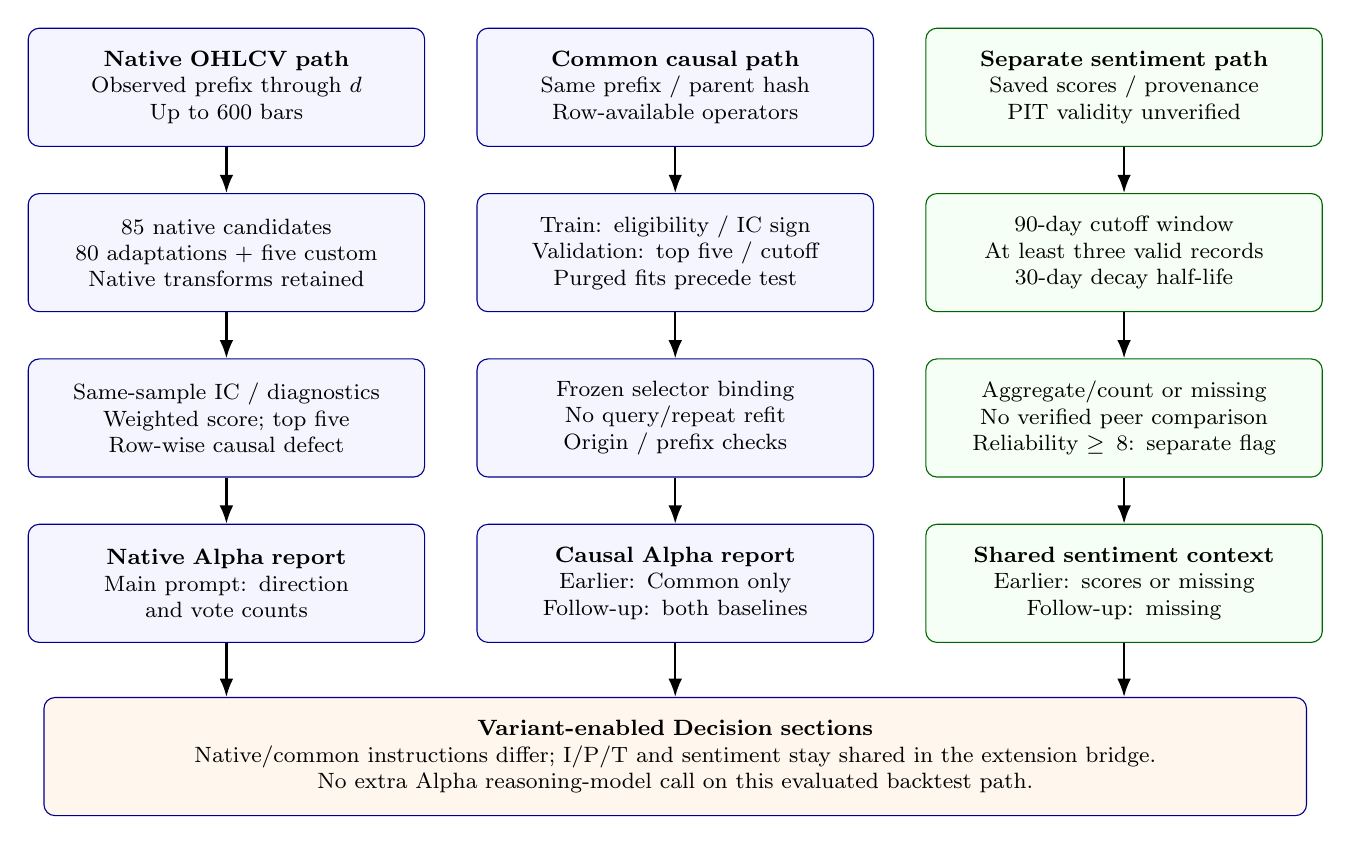
\begin{tikzpicture}[>=Latex,
 box/.style={draw=blue!55!black,fill=blue!4,rounded corners,align=center,text width=4.8cm,minimum height=1.5cm,font=\footnotesize},
 sent/.style={box,draw=green!40!black,fill=green!4},arr/.style={->,thick}]
\node[box] (n1) at (0,0) {\textbf{Native OHLCV path}\\Observed prefix through $d$\\Up to 600 bars};
\node[box] (c1) at (5.7,0) {\textbf{Common causal path}\\Same prefix / parent hash\\Row-available operators};
\node[sent] (s1) at (11.4,0) {\textbf{Separate sentiment path}\\Saved scores / provenance\\PIT validity unverified};
\node[box] (n2) at (0,-2.1) {85 native candidates\\80 adaptations + five custom\\Native transforms retained};
\node[box] (c2) at (5.7,-2.1) {Train: eligibility / IC sign\\Validation: top five / cutoff\\Purged fits precede test};
\node[sent] (s2) at (11.4,-2.1) {90-day cutoff window\\At least three valid records\\30-day decay half-life};
\node[box] (n3) at (0,-4.2) {Same-sample IC / diagnostics\\Weighted score; top five\\Row-wise causal defect};
\node[box] (c3) at (5.7,-4.2) {Frozen selector binding\\No query/repeat refit\\Origin / prefix checks};
\node[sent] (s3) at (11.4,-4.2) {Aggregate/count or missing\\No verified peer comparison\\Reliability $\ge8$: separate flag};
\node[box] (n4) at (0,-6.3) {\textbf{Native Alpha report}\\Main prompt: direction\\and vote counts};
\node[box] (c4) at (5.7,-6.3) {\textbf{Causal Alpha report}\\Earlier: Common only\\Follow-up: both baselines};
\node[sent] (s4) at (11.4,-6.3) {\textbf{Shared sentiment context}\\Earlier: scores or missing\\Follow-up: missing};
\foreach \a/\b in {n1/n2,n2/n3,n3/n4,c1/c2,c2/c3,c3/c4,s1/s2,s2/s3,s3/s4}{\draw[arr] (\a)--(\b);}
\node[box,text width=15.8cm,fill=orange!7] (out) at (5.7,-8.5) {\textbf{Variant-enabled Decision sections}\\Native/common instructions differ; I/P/T and sentiment stay shared in the extension bridge.\\No extra Alpha reasoning-model call on this evaluated backtest path.};
\foreach \n in {n4,c4,s4}{\draw[arr] (\n.south)--(\n.south |- out.north);}
\end{tikzpicture}

\caption{Native and causal alpha processing with separate Vietnamese sentiment context.}
\label{fig:alpha_agent}
\end{figure}

\subsection{Pattern Agent}
Pattern Agent analyses a candlestick PNG rendered with mplfinance \cite{mplfinance_docs} from the exact 45-bar window. The prompt requests a chart formation, recent-candle evidence, directional bias, confidence and trading implication. The report parser retains the structured text fields; format completion and consistency checks are distinguished from financial correctness. Figure~\ref{fig:charts} presents an actual archived chart pair rather than a synthetic demonstration.

Candle bodies are green when Close exceeds Open and red otherwise, including a doji. This is an Open--Close body rule, not the Vietnamese exchange board's reference-price colouring rule. The exchange-board convention is not used to infer candle direction. After inference, consistency rules compare the claimed bias with simple OHLCV-derived properties such as the final body and recent closes. A contradiction flag can reduce displayed confidence; it cannot reveal which candle the VLM actually attended to. The reported vision requests use their stored chart inputs.

\begin{figure}[htb]
\centering
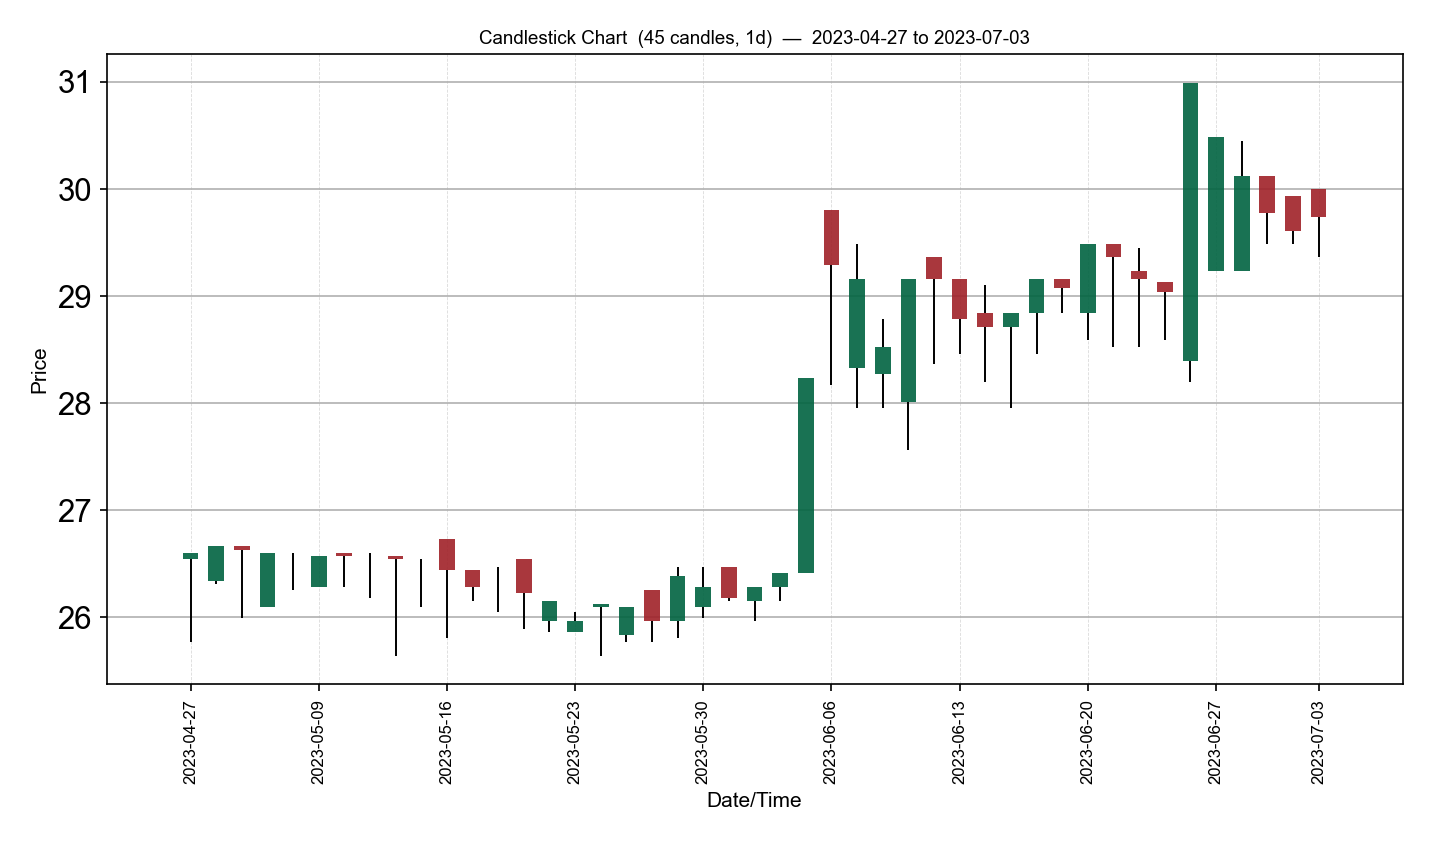
\includegraphics[width=0.90\textwidth]{figures/candlestick.png}\par\smallskip
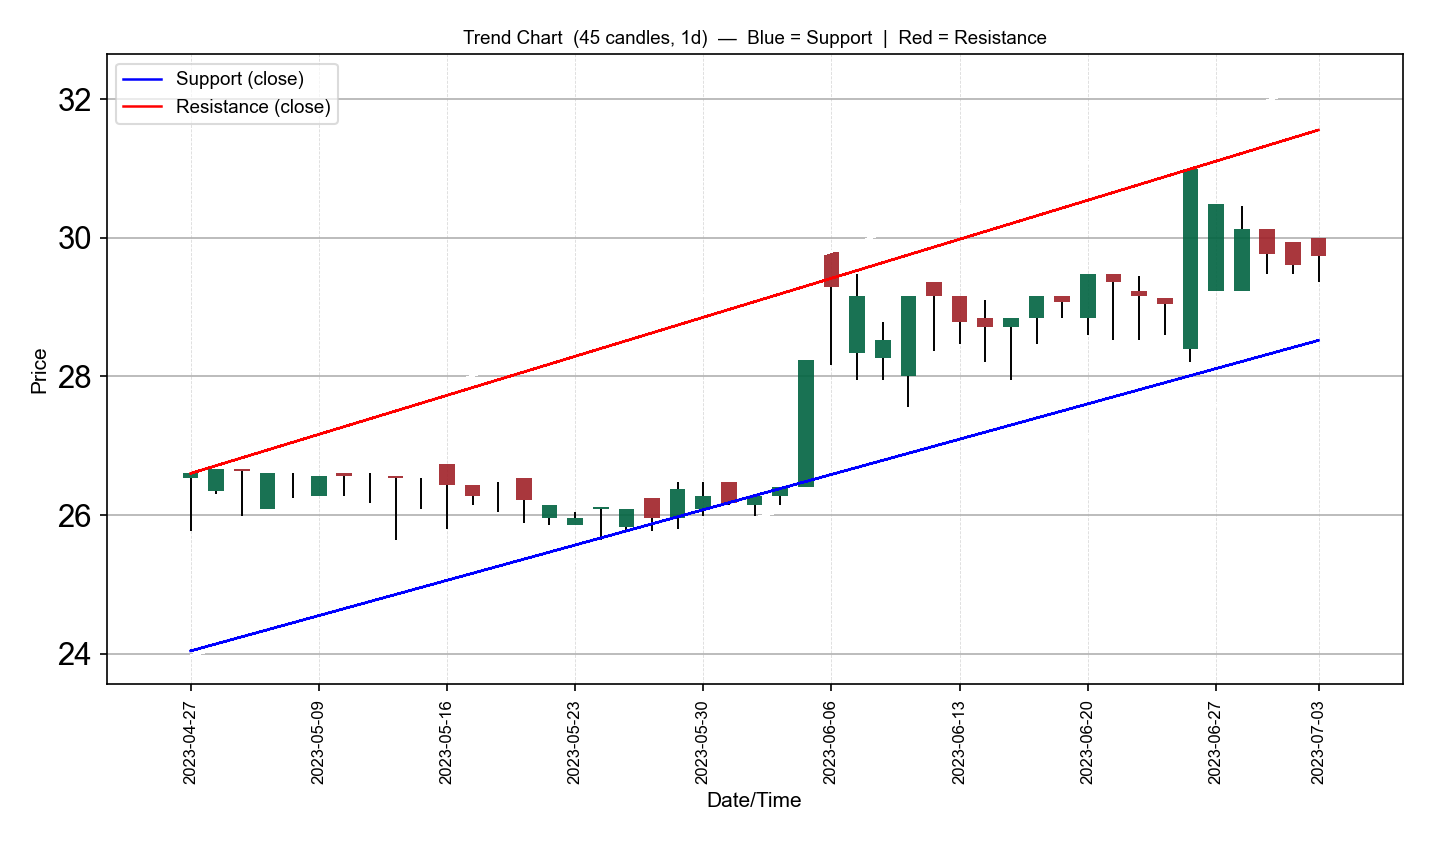
\includegraphics[width=0.90\textwidth]{figures/trendlines.png}
\caption{Candlestick and support--resistance inputs for CMG at the 3 July 2023 decision cutoff.}
\label{fig:charts}
\end{figure}

\subsection{Trend Agent}
Trend Agent receives a separate chart with fitted support/resistance lines. The inherited fitting utility starts with a least-squares close-price line, selects upper/lower deviation pivots, and optimizes a slope through each pivot under a non-crossing constraint. It implements both a close-only channel and a high/low channel, the latter using close-price regression to find pivots and high/low data for the bounds. These are numerical lines over the supplied window, not human-verified latent support levels.

For row position $u$, a fitted line has form $b+mu$. A support bound must remain below the corresponding price sequence within the implementation tolerance; resistance must remain above it. The local slope search reduces its step when the squared-deviation objective fails to improve or violates the constraint. The VLM then describes direction, levels, slope, price relative to support, forecast and confidence. Support is drawn blue and resistance red. A deterministic consistency check against simple price/trend summaries does not validate every reported level or coordinate.

Input checks match 204 chart images across 102 units byte for byte and pixel for pixel, and 240 recorded vision requests match their image caches and Vietnamese templates. The charts use blue support and red resistance lines, while the Vietnamese word \emph{xanh} is less colour-specific than the English term ``blue. Inherited high-frequency/K-line wording is used with daily bars, and the model's interpretation of these instructions is unverified.

\subsection{Decision Agent}
Decision receives condensed Indicator, Pattern and Trend reports plus enabled factor/sentiment sections. Reports are distilled and capped before prompt composition. The component study's observed successful Decision prompts are at most 4,187 characters, below the 6,500-character guard. Figure~\ref{fig:decision_agent} shows the extension dependencies, raw proposals, fallback and separate action policy.

\begin{figure}[htb]
\centering% Mũi tên giữa vai trò là dependency cùng repeat; policy tách raw/final.
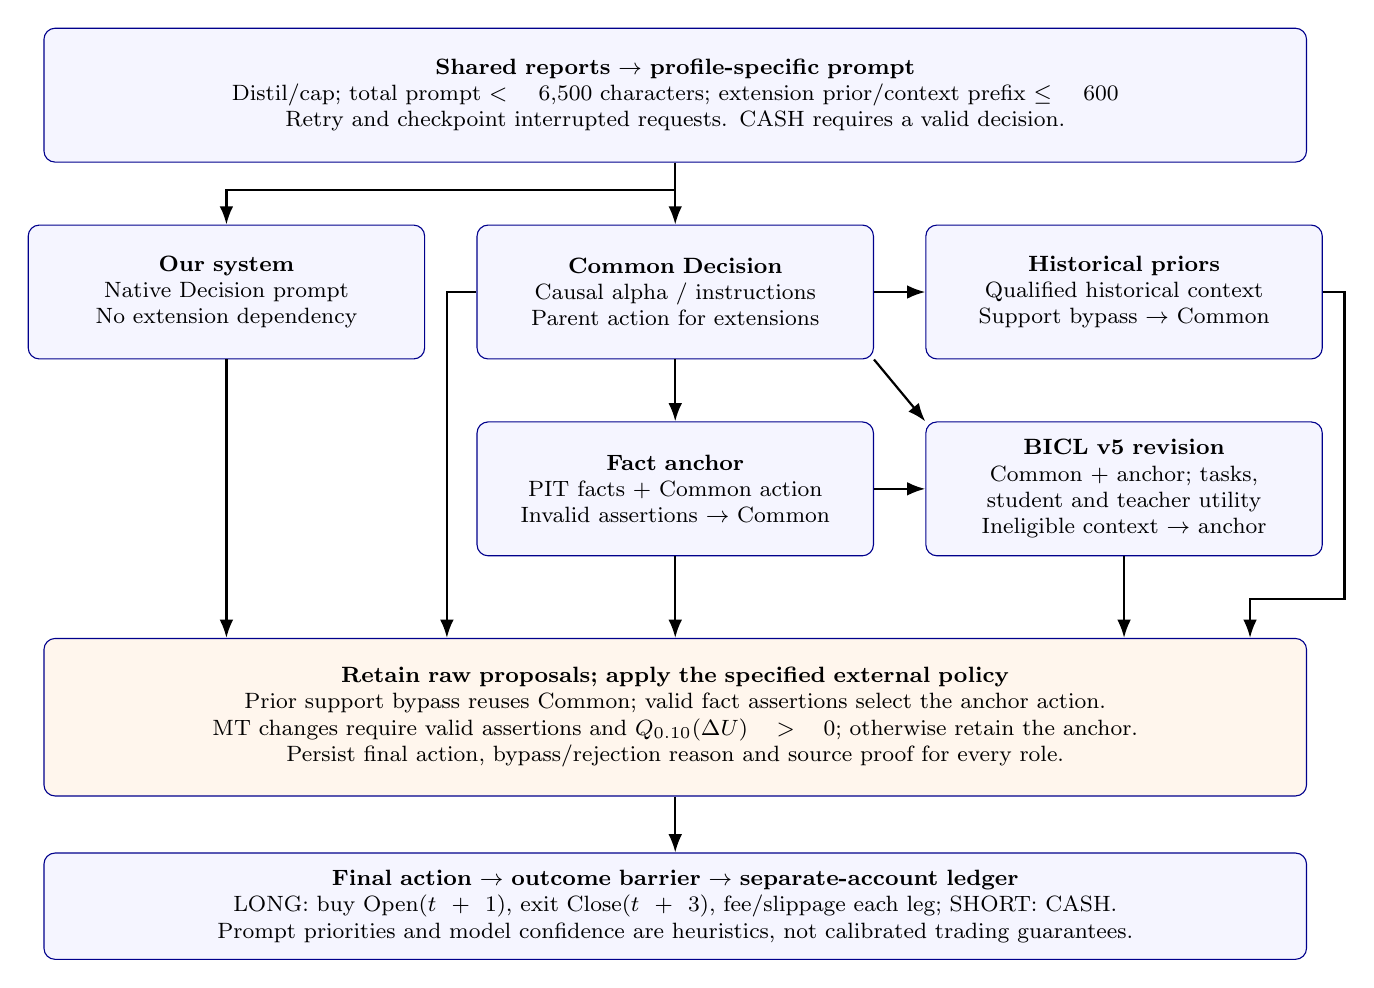
\begin{tikzpicture}[>=Latex,
 box/.style={draw=blue!55!black,fill=blue!4,rounded corners,align=center,text width=4.8cm,minimum height=1.7cm,font=\footnotesize},
 wide/.style={box,text width=15.8cm},arr/.style={->,thick}]
\node[wide] (in) at (5.7,0) {\textbf{Shared reports $\rightarrow$ profile-specific prompt}\\Distil/cap; total prompt $<6{,}500$ characters; extension prior/context prefix $\le600$\\Retry and checkpoint interrupted requests. CASH requires a valid decision.};
\node[box] (native) at (0,-2.5) {\textbf{Our system}\\Native Decision prompt\\No extension dependency};
\node[box] (common) at (5.7,-2.5) {\textbf{Common Decision}\\Causal alpha / instructions\\Parent action for extensions};
\node[box] (prior) at (11.4,-2.5) {\textbf{Historical priors}\\Qualified historical context\\Support bypass $\rightarrow$ Common};
\draw[arr] (in.south)--++(0,-0.35)-|(native.north);
\draw[arr] (in.south)--(common.north);
\draw[arr] (common.east)--(prior.west);
\node[box] (fact) at (5.7,-5) {\textbf{Fact anchor}\\PIT facts + Common action\\Invalid assertions $\rightarrow$ Common};
\node[box] (mt) at (11.4,-5) {\textbf{BICL v5 revision}\\Common + anchor; tasks,\\student and teacher utility\\Ineligible context $\rightarrow$ anchor};
\draw[arr] (common.south)--(fact.north);
\draw[arr] (common.south east)--(mt.north west);
\draw[arr] (fact.east)--(mt.west);
\node[wide,fill=orange!7,minimum height=2cm] (policy) at (5.7,-7.9) {\textbf{Retain raw proposals; apply the specified external policy}\\Prior support bypass reuses Common; valid fact assertions select the anchor action.\\MT changes require valid assertions and $Q_{0.10}(\Delta U)>0$; otherwise retain the anchor.\\Persist final action, bypass/rejection reason and source proof for every role.};
\draw[arr] (native.south)--(native.south |- policy.north);
\draw[arr] (common.west)--(2.8,-2.5)--(2.8,-6.8)--(2.8,-6.8 |- policy.north);
\draw[arr] (prior.east)--(14.2,-2.5)--(14.2,-6.4)--(13,-6.4)--(13,-6.4 |- policy.north);
\draw[arr] (fact.south)--(fact.south |- policy.north);
\draw[arr] (mt.south)--(mt.south |- policy.north);
\node[wide,minimum height=1.35cm] (ledger) at (5.7,-10.3) {\textbf{Final action $\rightarrow$ outcome barrier $\rightarrow$ separate-account ledger}\\LONG: buy Open$(t+1)$, exit Close$(t+3)$, fee/slippage each leg; SHORT: CASH.\\Prompt priorities and model confidence are heuristics, not calibrated trading guarantees.};
\draw[arr] (policy)--(ledger);
\end{tikzpicture}

\caption{Decision dependencies, fallback rules and final-action policy.}
\label{fig:decision_agent}
\end{figure}

The instructions ask for trend/key-level assessment, recent-candle evidence, momentum confirmation and comparison with enabled factor/sentiment context. Price/chart evidence has priority, quantitative factors may challenge it, and sentiment has lower priority. These instructions describe an intended analysis sequence; they are not an independently observed internal reasoning trace or a guaranteed conflict-resolution algorithm.

The required output includes a binary LONG/SHORT forecast, forecast horizon, confidence, risk/reward field, evidence for/against and justification. Model confidence and risk/reward statements do not constitute calibrated uncertainty or executable price levels. In the long-only reference ledger, SHORT maps to CASH and LONG to the specified next-open/target-close cycle. The classifier's labels and account execution remain distinct.

Base retains the same upstream content and general instructions but removes both alpha and sentiment sections; those concepts may still appear in general instructions. Thus Full--Base changes a bundle and prompt length, not solely one numerical factor. Main/upstream prompts use compact factor text, whereas factorial A/AS/P deliver five explicit rows. The resulting representation difference remains part of the interpretation of the separate panels.

\paragraph{Historical-prior methods}
The \emph{Bayesian prior} (Bayesian in tables) retrieves up to three matured same-stock examples using regime and report-signal context. The \emph{conditional prior} (Conditional) adds Beta-based statistics matched on Trend/Pattern/Alpha/Indicator states, disjoint-background shrinkage and separate readiness checks for statistics and examples. The \emph{trend--pattern prior} (Trend--pattern) relaxes the statistics match to Trend/Pattern. The \emph{explicit-count prior} (Explicit counts) uses the conditional prior's support but explains counts, intervals and example identifiers more explicitly. Historical rates and plug-in intervals summarize the selected history; when no qualified prior is available, the method reuses Common's action for that repeat.

\paragraph{Fact anchor and MT-BICL}
Fact anchor receives a deterministic point-in-time fact packet, including MACD-versus-signal and Close-versus-SMA20 assertions, and the completed Common decision. Valid assertions select its proposed action without the numerical utility veto; invalid assertions select Common with a source proof. MT-BICL constructs numerical prior/target tasks conditioned on the factual bucket, retains a frozen student estimate and teacher-based utility summary, and requests a revision of that anchor only when context is eligible. The external policy in Eq.~\ref{eq:revision_utility} decides whether a changed proposal is accepted. Raw proposals, anchor actions, bypass and final actions are distinct saved fields, so final outcome differences cannot be assigned entirely to the LLM or student.

All extension prompts preserve report distillation/capping, require fewer than 6,500 characters and cap their prior/context prefix at 600 characters. The component-study maximum of 4,187 characters above is not an extension-run maximum. Exact prompt projections, readiness thresholds and request schemas are given in \ref{app:prompts} and~\ref{app:state_schema}; runtime resources and restore instructions are in \ref{app:software}.
\FloatBarrier

\section{Experimental Setup}
\label{sec:experimentalsetup}

\subsection{Dataset and Point-in-Time Data Contract}
The daily universe spans information technology (FPT, CMG), banking (VCB, MBB), retail (MWG), food/beverages (VNM, BHN) and aviation/tourism (HVN, VJC). The reconstructed VCI snapshot via vnstock~\cite{vnstock_docs} covers observed vendor sessions from 2020 through September 2026. The sample is purposive, and original historical data availability is unverified. A valid-suffix policy excludes contradictory BHN OHLC data; insufficient warm-up then excludes BHN from three early blocks. This leaves 102 eligible stock--date observations for the paired comparisons.

\paragraph{Component study, historical context and follow-up}
The component study uses the native alpha selector's compact consensus
and saved sentiment summaries or missingness, with QuantAgent omitting
both reports. It uses no historical retrieval. The earlier BICL study
compares native alpha in Our system with a frozen causal projection in
Common. The two share chart reports and the saved sentiment aggregate
or missingness flag. Historical retrieval uses the saved categorical
Trend and Pattern signals where required. Sentiment is missing at
\UnifiedMissingSentiment/\UnifiedPoints\ points in this collection.

The follow-up binds the same frozen causal alpha projection to Our
system and Common and keeps their distinct Decision prompts. It uses
a rebuilt OHLCV bank. Its Trend and Pattern retrieval keys are computed
from the same 45-session rule for query and bank. The chart-based
reports still enter Decision. No news meets the availability criterion
at the follow-up cutoffs. The reference action is Common for BICL
v1--v4 and Fact Anchor for BICL v5.

\subsection{Walk-Forward Protocol}
Six blocks cover 2023 H2, 2024 H2, 2025 H1, 2025 Q4, 2026 Q2 and 2026 Q3, with two scheduled dates per block. The sparse walk-forward schedule~\cite{pardo2008evaluation} shares dates across stocks. Each of the 51 eligible stock--block scopes splits train, validation and test chronologically and purges labels whose exit reaches the next partition.

The evaluation schedule was finalized after some inference, making this an exploratory historical analysis. The 375 component-study Decisions comprise 193 reused successful executions and 182 additional successes. The upstream panel shares 18 calls with the main comparison, so 204+54+135-18=375 unique Decisions. Factorial units were selected by stock/date round-robin metadata. Table~\ref{tab:scope} reports the supports of the main, upstream and factorial panels.

\begin{table}[!htb]
\centering\small
\setlength{\tabcolsep}{3pt}
\renewcommand{\arraystretch}{1.15}
\caption{Evaluation panels and enabled prompt components in the component study.}
\label{tab:scope}
\textbf{A. Recorded supports}\par\smallskip
\begin{tabular}{lrrrrrrr}
\hline
Scope & $N$/exec. & Symbols & Dates & Blocks & UP/DOWN & Exec. & Decisions \\
\hline
Main & 102 & 9 & 12 & 6 & 25/77 & 1 & 204 \\
Upstream & 9 & 9 & 3 & 3 & 2/7 & 3 & 54 \\
Factorial & 9 & 8 & 4 & 3 & 2/7 & 3 & 135 \\
\hline
\end{tabular}\par\medskip
\textbf{B. Prompt sections}\par\smallskip
\begin{tabular}{llll}
\hline
Variant & Factors & Sentiment & Representation \\
\hline
B & -- & -- & Shared price reports \\
A & Current & -- & Five-row factorial \\
S & -- & Current & Factorial \\
AS & Current & Current & Compact main / five-row factorial \\
P & Past donor & Current & Five-row factorial \\
\hline
\end{tabular}\par\medskip
\begin{minipage}{\textwidth}\footnotesize B omits both components, A enables factors, S enables sentiment, AS enables both, and P replaces current factors with a past training donor.\end{minipage}
\end{table}


The extension fixes \UnifiedPoints\ points, \UnifiedAccounts\ symbol--fold accounts, \UnifiedUpstreamRealizations\ upstream realization per point and \UnifiedDecisionRepeats\ Decision repeats. One immutable report/image parent is deep-copied into all roles; each repeat uses new Decision responses where a call is eligible. The \UnifiedForecastSlots\ research slots are not independent market samples, full-system executions or successful HTTP calls. All 102 evaluation IDs are reserved globally before context labels can be computed, including IDs belonging to earlier folds. Context is frozen before the first test query in a fold and reused at its second anchor; test labels are never added prequentially.
\begin{table}[!htb]
\centering\small
\setlength{\tabcolsep}{3pt}
\renewcommand{\arraystretch}{1.12}
\caption{Market coverage and execution counts in the historical-context study.}
\label{tab:u09-scope}
\textbf{Recorded support}\par\smallskip
\begin{tabular}{lr}
\hline
Quantity & Count \\
\hline
Market points & 102 \\
Symbols & 9 \\
Dates & 12 \\
Folds & 6 \\
Independent-capital accounts per repeat & 51 \\
Upstream realizations per point & 1 \\
Upstream executions & 102 \\
Points without available sentiment & 79 \\
Decision repeats & 3 \\
Research forecast slots (eight roles) & 2448 \\
Raw Decision responses & 1290 \\
HTTP attempts (including retired) & 1702 \\
\hline
\end{tabular}\par\medskip
\begin{minipage}{\textwidth}\footnotesize BHN contributes six points in three folds, other stocks twelve each; repeats share one upstream realization per point.\end{minipage}
\end{table}


\begin{figure}[!htb]
\centering% Cutoff/context và hàng rào outcome; không đưa nhãn query vào prompt.
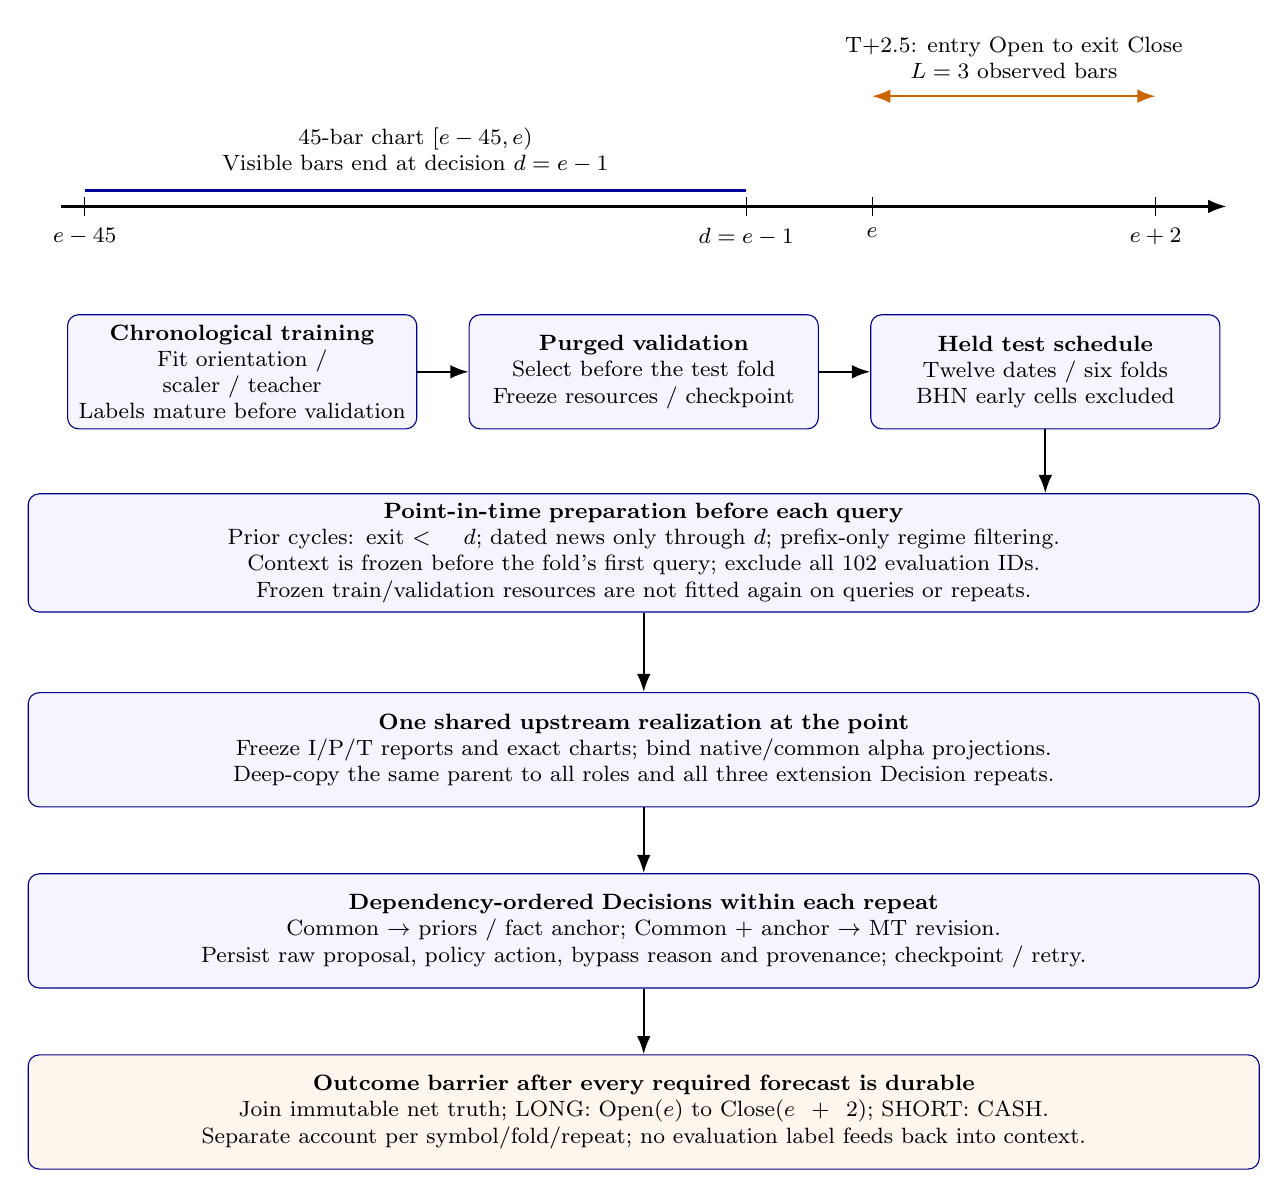
\begin{tikzpicture}[>=Latex,
 box/.style={draw=blue!55!black,fill=blue!4,rounded corners,align=center,text width=4.2cm,minimum height=1.45cm,font=\footnotesize},
 wide/.style={box,text width=15.4cm},arr/.style={->,thick}]
\draw[->,thick] (-0.3,0)--(14.5,0);
\draw[very thick,blue!60!black] (0,0.2)--(8.4,0.2);
\node[above,align=center,font=\footnotesize] at (4.2,0.3) {45-bar chart $[e-45,e)$\\Visible bars end at decision $d=e-1$};
\foreach \x/\lab in {0/{e-45},8.4/{d=e-1},10/{e},13.6/{e+2}}{\draw (\x,-0.12)--(\x,0.12);\node[below,font=\footnotesize] at (\x,-0.15) {$\lab$};}
\draw[<->,thick,orange!80!black] (10,1.4)--(13.6,1.4);
\node[above,align=center,font=\footnotesize] at (11.8,1.5) {T+2.5: entry Open to exit Close\\$L=3$ observed bars};
\node[box] (train) at (2,-2.1) {\textbf{Chronological training}\\Fit orientation / scaler / teacher\\Labels mature before validation};
\node[box] (valid) at (7.1,-2.1) {\textbf{Purged validation}\\Select before the test fold\\Freeze resources / checkpoint};
\node[box] (test) at (12.2,-2.1) {\textbf{Held test schedule}\\Twelve dates / six folds\\BHN early cells excluded};
\draw[arr] (train)--(valid);\draw[arr] (valid)--(test);
\node[wide] (context) at (7.1,-4.4) {\textbf{Point-in-time preparation before each query}\\Prior cycles: exit $<d$; dated news only through $d$; prefix-only regime filtering.\\Context is frozen before the fold's first query; exclude all 102 evaluation IDs.\\Frozen train/validation resources are not fitted again on queries or repeats.};
\draw[arr] (test.south)--(test.south |- context.north);
\node[wide] (shared) at (7.1,-6.9) {\textbf{One shared upstream realization at the point}\\Freeze I/P/T reports and exact charts; bind native/common alpha projections.\\Deep-copy the same parent to all roles and all three extension Decision repeats.};
\draw[arr] (context)--(shared);
\node[wide] (decision) at (7.1,-9.2) {\textbf{Dependency-ordered Decisions within each repeat}\\Common $\rightarrow$ priors / fact anchor; Common + anchor $\rightarrow$ MT revision.\\Persist raw proposal, policy action, bypass reason and provenance; checkpoint / retry.};
\draw[arr] (shared)--(decision);
\node[wide,fill=orange!7] (out) at (7.1,-11.5) {\textbf{Outcome barrier after every required forecast is durable}\\Join immutable net truth; LONG: Open$(e)$ to Close$(e+2)$; SHORT: CASH.\\Separate account per symbol/fold/repeat; no evaluation label feeds back into context.};
\draw[arr] (decision)--(out);
\end{tikzpicture}

\caption{Chronological data preparation, shared inference and T+2.5 execution.}
\label{fig:walkforward}
\end{figure}

\subsection{Paired Baseline and Disentangled Ablations}
Our system and QuantAgent share the 102 cutoffs, technical reports,
net outcome labels and costs. The main compact Our system prompt includes
a five-factor direction and bullish, bearish and neutral vote counts.
The saved Decision requests contain individual factor-value rows at
0/102 cutoffs and mark sentiment as missing at 79/102. The separate
factorial panel sends individual rows. Table~\ref{tab:classification}
also includes logistic-price, a price-only classifier using the saved
purged train/validation fit and threshold, and CASH, which stays flat.
Both controls use the same cutoffs and account definitions.

The comparison includes differences in report wording, prompt length and trading frequency. The upstream panel has nine units, B/AS and three regenerated upstream realizations with a Decision execution per realization. The factorial panel has nine different-support units, B/A/S/AS/P and three Decision executions with fixed upstream. Both have two UP/seven DOWN per execution, but only the former covers nine symbols. We do not infer main-grid variability or separate upstream/Decision variance components from their SDs.

P retains current factor names, headings, schema/missingness and sentiment, replacing scalar values, signals and skill fields using a predetermined earlier train-only rank-vector donor. Donor label exits precede validation/test. Rank mapping is not name-matched covariance preservation, a placebo distribution or exposure matching. Five explicit rows reach each A/AS/P factorial prompt. Main/upstream compact prompts are a separate representation family. Interaction is defined as $AS-A-S+B$; the observed best-single gap $AS-\max(A,S)$ is a different, post-hoc diagnostic and not an eighth factorial contrast.

\paragraph{Historical-context comparators}
This study compares BICL v1--v5 with Our system and Common and uses Fact Anchor to examine the revision step. Each of the five methods is compared with Our system in the system family and with Common in the method family. Fact Anchor is a dependency and control. Three additional comparisons describe Common versus Our system, Fact Anchor versus Common, and BICL v5 versus Fact Anchor; these are outside the primary contrast families. The nine-unit upstream/factorial panels evaluate component interventions on separate observation sets.

\subsection{Account and Statistical Metrics}
Balanced accuracy (BA)~\cite{brodersen2010balanced}, Matthews correlation coefficient (MCC)~\cite{chicco2020mcc} and per-class precision and recall accompany ordinary accuracy and LONG rate. Main contrasts use dependent-data resampling~\cite{lahiri2003resampling} with 10,000 paired whole-block resamples, seed 20261102, retaining dates, cross-section, variants and eligibility together. Repeat diagnostics jointly resample recorded blocks and paired execution indices. Intervals condition on finite draws; undefined counts remain visible. Circular block lengths, leave-one-block-out and Bartlett HAC~\cite{newey1987hac} at lags 0/1/2 are sensitivity diagnostics. HAC uses calendar-aligned accuracy differences in fixed-universe panels, with a $t(n_{dates}-1)$ reference; few clusters, irregular gaps and post-inference additions prevent calibrated significance or power claims.

To specify the classification estimand, let TP/FN count UP outcomes and TN/FP count DOWN outcomes. We use
\begin{equation}
 \begin{aligned}
 BA&=\frac12\left(\frac{TP}{TP+FN}+\frac{TN}{TN+FP}\right),\\
 MCC&=\frac{TP\,TN-FP\,FN}{\sqrt{(TP+FP)(TP+FN)(TN+FP)(TN+FN)}}.
 \end{aligned}
 \label{eq:classification_metrics}
\end{equation}
The relevant metric is undefined when a required denominator is zero. Macro means average defined symbol-level values while retaining the planned and defined denominators.

Each of 51 symbol--block accounts starts with VND50 million, without cross-symbol capital competition. LONG follows Eq.~\ref{eq:label}; CASH stays flat. Wealth includes pending receivables and residual shares at recorded mark-to-market prices. Daily-close drawdown uses an initial-capital anchor. Daily Sharpe~\cite{sharpe1966mutual} uses population SD, 252 sessions and a zero risk-free rate. Daily Sortino~\cite{sortino1994downside} in the companion uses the SD of negative daily observations. Irregular spacing precludes annualizing cycle ratios.

The T+2.5 reference assumes fractional fills at recorded prices and two-leg fees and slippage. Sale proceeds stay pending until the specified settlement phase. The fixed cycle covers \(L=3\) observed bars, including entry. Daily OHLC cannot authenticate opening-auction queues, price-limit fills, partial fills or correct volume units. Selected execution sensitivities appear in \ref{app:additional}. Ten HVN stock--date observations have unresolved venue/calendar consistency flags.

\paragraph{Historical-context metrics}
In the historical-context study, each method has three independent-capital executions per stock--fold account. Returns are averaged across repeats within account and then equally over 51 accounts; BA is computed separately on 102 points per repeat and then averaged. Evaluated predictions follow final policy actions. Daily EOD NAV, cycle drawdown, costs, turnover and held-session fraction retain their own units. Cycle Sharpe uses sample SD (ddof=1); cycle Sortino uses the RMS of negative-part returns over all cycles with MAR zero. The irregular schedule does not support annualized ratios. Metrics with zero or missing denominators are left blank in the analysis.

The extension uses paired circular fold bootstrap draws with block length two, 10,000 draws, PCG64 seed 20261110, retaining cross-section, eligibility and all methods/repeats together. Identical resample indices serve all twenty return/BA endpoint contrasts in the two specified families. Simultaneous descriptive bands use standardized maximum deviation across those twenty columns. Finite/null rules apply jointly; draws are not redrawn to hide an undefined endpoint, and a degenerate family does not receive substitute bands. L1/L3, leave-one-fold-out, leave-one-symbol-out and the bank-covered subset remain sensitivity analyses. These six historically exposed folds do not establish calibrated coverage, significance or power. The component-study seed, estimands and finite-draw conventions remain unchanged.

\subsection{Implementation and Robustness Design}
Archived SDK aliases are \texttt{openai/gpt-oss-20b} for text and \texttt{qwen/qwen3.8-27b} for vision. Configured temperature zero appears as $10^{-8}$ in observed SDK metadata; no hosted decoding seed is recorded. Text/vision output caps are 2,048/1,024 tokens. Retry/checkpoint records preserve individual attempts and completed outputs. Aliases and 40 response fingerprints do not authenticate an immutable weight revision or historical provider catalogue; 91 original Pattern requests lack provider organization and execution-epoch records. Offline replay reproduces saved-prediction metrics, not a fresh hosted inference experiment.

The component-study execution records contain 649 attempts, 615 successes and 34 errors, including 120 shared Pattern calls. Observed usage totals 1,063,328 prompt and 340,736 completion tokens; the ledger has no usage or latency for interrupted requests and no monetary billing. Recorded callback elapsed times exclude unobserved waiting and do not measure wall-clock runtime.

\paragraph{Historical context and execution resources}
The historical-context study fixes prompts, aliases, decoding options and dependency order before its own execution. Retry handling allows three total attempts including schema repair, with durable checkpoints and reconciliation of uncertain requests. Records contain 1,702 HTTP attempts, including 15 superseded attempt records, and 1,290 active raw Decision responses. These counts refer to attempts and responses respectively and remain separate from the component-study totals.

The prior bank contains 852 fixed historical examples for FPT, MWG, VCB and VNM; the other five stocks follow the specified support/fallback policy. Bank and query inputs have separate provenance. Numeric MT context, scaler, HMM and teacher are fixed with student checkpoint seed 42/step 3000, and all 51 causal alpha selectors are fitted before their queries. Inference uses these resources without refitting.

\section{Backtest Results}
\label{sec:backtestresults}

\subsection{Nine-Symbol Paired Benchmark}
\subsubsection{Directional forecasts and account returns}
On the 102 paired observations, Our system identifies seven of 25 UP
outcomes, as does QuantAgent. It issues five fewer false LONG forecasts
(17 versus 22), which raises balanced accuracy by \DeltaBA{} percentage
points. The paired descriptive interval is $[\PrimaryLow,\PrimaryHigh]$
pp. Table~\ref{tab:classification} reports the pooled forecast metrics and
the mean outcomes of 51 separate accounts per system.

\begin{table}[!htb]
\centering\small
\setlength{\tabcolsep}{6pt}
\renewcommand{\arraystretch}{1.13}
\caption{Main component-study results at 102 paired cutoffs and 51 accounts per method.}
\label{tab:classification}
\begin{tabular}{@{}lrrrrrr@{}}
\toprule
& \multicolumn{3}{c}{Forecasts} & \multicolumn{3}{c}{Accounts}\\
\cmidrule(lr){2-4}\cmidrule(lr){5-7}
Method & Acc. (\%) & BA (\%) & LONGs & Net return (\%) & MDD (\%) & Held (\%)\\
\midrule
Our system & 65.69 & 52.96 & 24 & -0.797 & 1.37 & 2.35\\
QuantAgent & 60.78 & 49.71 & 29 & -0.750 & 1.45 & 2.84\\
Logistic-price & 67.65 & 55.61 & 24 & -0.683 & 1.18 & 2.35\\
CASH & 75.49 & 50.00 & 0 & 0.000 & 0.00 & 0.00\\
\bottomrule
\end{tabular}
\par\smallskip
{\footnotesize BA is balanced accuracy. MDD is mean maximum daily-close drawdown.
Held is the mean share of observed sessions spent invested.\par}
\end{table}


Our system has lower drawdown on average and spends less time invested
(2.35\% of observed sessions, versus 2.84\%). Its mean net return is
nevertheless 0.047 pp lower. Balanced accuracy weights the two classes
equally, whereas returns depend on the size and timing of the selected
trades. The comparison measures the contribution of the two added reports
and the augmented Decision prompt together.

\subsubsection{Historical-context comparison}
Table~\ref{tab:u09-comparison} reports the earlier evaluation of BICL and
both augmented-system baselines. BICL v1 improves mean return versus
Common by $+\UnifiedVOneCommonReturnEffect$ pp, with a descriptive band of
$[\UnifiedVOneCommonReturnLow,\UnifiedVOneCommonReturnHigh]$ pp. Its
difference versus Our system is $\UnifiedVOneNativeReturnEffect$ pp, with
a band of $[\UnifiedVOneNativeReturnLow,\UnifiedVOneNativeReturnHigh]$ pp.
Figure~\ref{fig:u09-return-contrasts} shows the corresponding differences
for all five versions.

\begin{table}[htb]
\centering\small
\setlength{\tabcolsep}{3pt}
\renewcommand{\arraystretch}{1.12}
\caption{Mean returns, balanced accuracy and support across historical-context methods and controls.}
\label{tab:u09-comparison}
\textbf{Paired support: 102 points per repeat}\par\smallskip
\begin{tabular}{lrrrrrr}
\hline
Role & Return (\%) & BA (\%) & LONG (\%) & Raw & Bypass & $N$/repeat \\
\hline
Our system & -0.653 & 51.84 & 22.55 & 306 & 0 & 102 \\
Our system (Common) & -1.025 & 45.97 & 28.76 & 306 & 0 & 102 \\
BICL v1 & -0.698 & 50.10 & 23.86 & 144 & 162 & 102 \\
BICL v2 & -1.030 & 45.75 & 29.08 & 3 & 303 & 102 \\
BICL v3 & -1.019 & 46.18 & 28.43 & 24 & 282 & 102 \\
BICL v4 & -1.030 & 45.75 & 29.08 & 3 & 303 & 102 \\
BICL v5 & -1.253 & 43.17 & 34.31 & 198 & 108 & 102 \\
Fact Anchor & -1.286 & 42.74 & 34.97 & 306 & 0 & 102 \\
CASH & 0.000 & 50.00 & 0.00 & 0 & 306 & 102 \\
Always-LONG & -3.000 & 50.00 & 100.00 & 0 & 306 & 102 \\
\hline
\end{tabular}\par\medskip
\begin{minipage}{\textwidth}\footnotesize Return averages 51 accounts after averaging three repeats; BA averages per-repeat metrics, and Raw/Bypass counts cover 306 method slots.\end{minipage}
\end{table}


\begin{figure}[b]
\centering
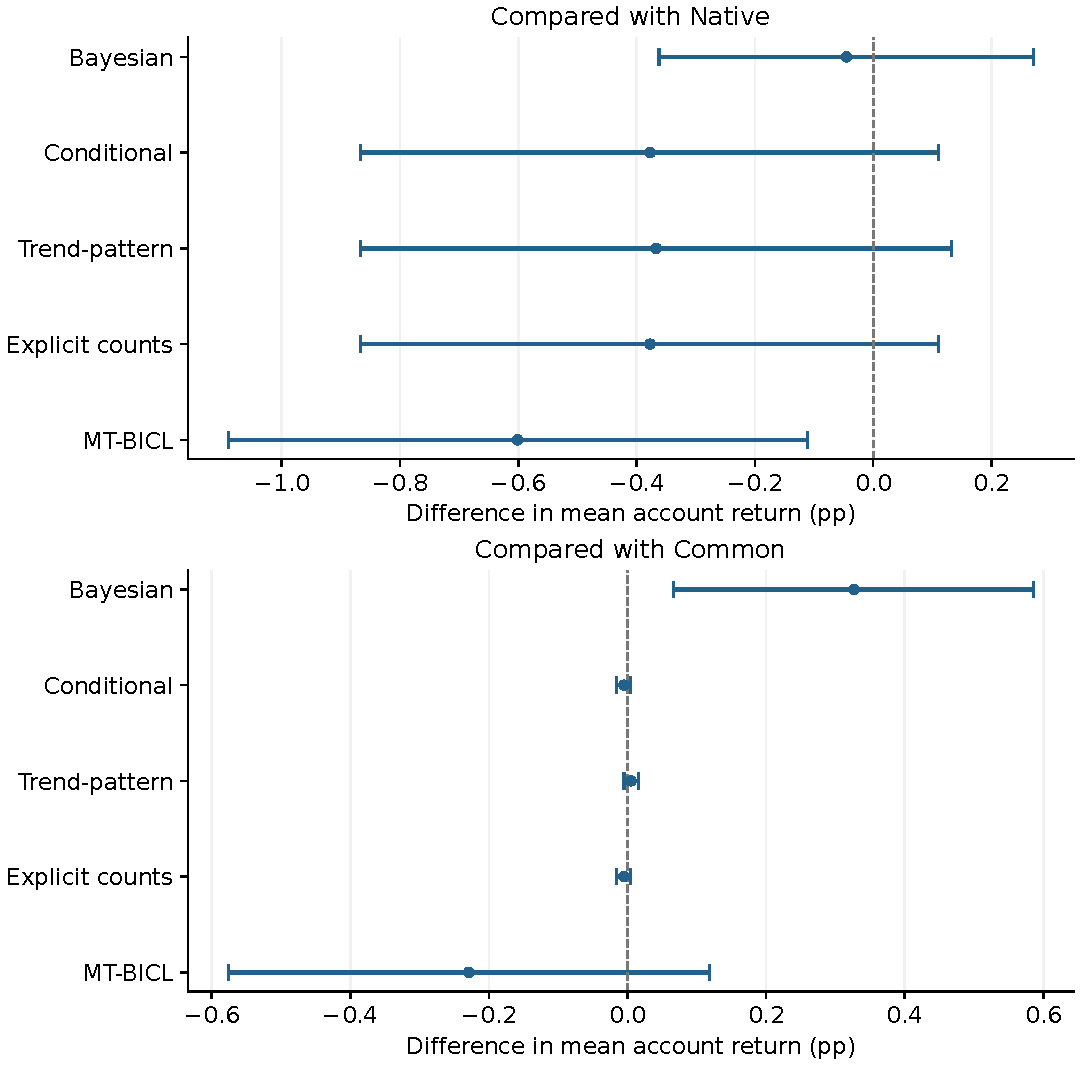
\includegraphics[width=0.84\textwidth,height=.40\textheight,keepaspectratio]{figures/return_comparisons.pdf}
\caption{Earlier historical-context study. Mean account-return differences against each augmented-system baseline, with descriptive simultaneous bands.}
\label{fig:u09-return-contrasts}
\end{figure}

BICL v2 and v4 each request only three new decisions across 306 slots.
Consequently, their aggregate outcomes mostly reflect fallback to Common.
BICL v5 agrees with Fact Anchor on 302 of 306 final actions. The three
successive comparisons in Table~\ref{tab:u09-bridge} show how much each
policy change affected actions and outcomes.

\paragraph{Follow-up historical-context evaluation}
The follow-up uses the same 102 cutoffs, a common causal alpha projection
and a rebuilt OHLCV memory bank. No news meets the historical
availability criterion on those dates. Five holding periods cross a
corporate action and one required entry has zero matched volume. Table%
~\ref{tab:bicl-complete-accounts} therefore compares the 45 accounts per
repeat with two labeled cycles, covering 90 cutoffs per repeat.

% Chiếu từ kết quả đã khóa của lần đánh giá bổ sung.
\begin{table}[!htb]
\centering\small
\caption{Follow-up BICL comparison on accounts with both trading cycles.}\label{tab:bicl-complete-accounts}
\begin{tabular}{lrrr}\toprule
Method & Mean net return (\%) & Balanced accuracy (\%) & Fallbacks / 306 \\ \midrule
Our system & -0.9379 & 46.2121 & 0 \\
Our system (Common) & -0.5304 & 53.2828 & 0 \\
BICL v1 & -0.5315 & 52.3990 & 162 \\
BICL v2 & -0.5177 & 53.7879 & 300 \\
BICL v3 & -0.5304 & 53.2828 & 282 \\
BICL v4 & -0.5177 & 53.7879 & 300 \\
BICL v5 & -1.0600 & 44.3182 & 117 \\
Fact Anchor & -1.0257 & 45.0758 & 0 \\
\bottomrule\end{tabular}
\par\smallskip
{\footnotesize Each repeat includes 45 of 51 accounts with both cycles, covering 90 cutoffs shared by all methods. Across the full sample, 96 of 102 cutoffs have valid execution labels.\par}
\end{table}


Mean-return differences for BICL v1--v4 versus Common range from
$-0.0011$ to $+0.0127$ pp. BICL v5 returns $-1.0600$\%, or $-0.1221$
and $-0.5297$ pp relative to Our system and Common, respectively.
The comparison uses owner-attested prices. The timing of historical
availability still needs independent verification.

\subsection{Component Contrasts and Variability}
Table~\ref{tab:repeats} reports a panel that regenerates chart reports and
a separate panel that holds the reports fixed while changing the
evidence shown to Decision. Each uses nine observations and three
executions. With a fixed upstream, the two-report branch trails
QuantAgent by 9.52 pp in balanced accuracy and the donor-value
variant by 11.90 pp. All seven descriptive factorial intervals include
zero. With regenerated reports, the paired difference is $+4.76$ pp
with a descriptive percentile interval of $[0,10]$ pp. The panels use
different cutoffs and cannot be combined to estimate variability for
the main 102-point cohort.

\begin{table}[!htb]
\centering\small
\renewcommand{\arraystretch}{1.13}
\caption{Component comparisons in two nine-observation panels. Cells are mean and sample SD across three executions.}
\label{tab:repeats}
\begin{tabular}{@{}llrr@{}}
\toprule
Panel & Method & BA (\%) & Net return (\%)\\
\midrule
Regenerated reports & QuantAgent & $90.48\pm 10.91$ & $0.37\pm 0.38$\\
 & Our system & $95.24\pm 4.12$ & $0.50\pm 0.22$\\
\addlinespace
Fixed reports & QuantAgent & $28.57\pm 7.14$ & $-1.70\pm 0.55$\\
 & Alpha only & $19.05\pm 4.12$ & $-2.03\pm 0.31$\\
 & Sentiment only & $14.29\pm 0.00$ & $-2.34\pm 0.22$\\
 & Our system & $19.05\pm 10.91$ & $-2.23\pm 0.63$\\
 & Past-donor alpha and sentiment & $30.95\pm 4.12$ & $-1.42\pm 0.33$\\
\bottomrule
\end{tabular}
\end{table}


\subsection{Robustness and Sensitivity}
Balanced accuracy varies across stocks and cutoffs
(Table~\ref{tab:symbol_results}). VNM has only DOWN observations, so
stock-level balanced accuracy is omitted there. On the common eight
stocks, the Our system--QuantAgent BA difference is $+2.08$ pp on 96
observations. Restricting the comparison to the three recent blocks
gives $+6.41$ pp on 54 observations. These overlapping cohorts share
dates and shocks.

Execution assumptions can change the return ordering. Higher costs
reverse the ordering under the reference ledger (Table~\ref{tab:execution}).
The additional comparisons in \ref{app:additional} use the same paired
forecasts. Repeated Decision calls and resampling quantify variability
conditional on the recorded dates and upstream realization.

\section{Limitations and Future Work}
\label{sec:limitations}

\subsection{Limitations}
\paragraph{Component attribution}
Our system--QuantAgent changes factor and sentiment content together with prompt length. Compact reports in the main/upstream panel also differ from the explicit factor rows in the factorial panel. The placebo uses one predetermined past donor, and only nine market units support each repeated component panel. These differences limit attribution of forecast changes to specific information sources. The evaluations lack matched ablations for retrieval, statistics, prior tasks, target tasks and utility.

\paragraph{Factor construction and sentiment validity}
Our system backward filling, whole-Series normalization and volume-availability branching can make an earlier historical row depend on later rows within the supplied prefix. Isolation from prices after the current decision cutoff therefore coexists with noncausal historical diagnostics. Our system orientation and ranking also reuse their calibration observations. The causal projection fits orientation and selection before testing. Six selected metadata slots differ from their handler descriptions, and the semantic effect of these mismatches is unmeasured.

Historical news content and publication availability are not independently authenticated, and no financial-domain sentiment test set or annotation agreement is available. Legacy scores without a recorded scorer and locally rescored excerpts come from distinct sources. Missing sentiment, including 79/102 historical-context points, reduces the information actually available to the methods. Bank and query return calculations also differ numerically in 828/852 bank records, with maximum absolute discrepancy about 0.042988489 percentage points; this comparison concerns returns rather than a count of label changes.

\paragraph{Sampling and model variability}
The nine equities form a purposive sample with unverified point-in-time listing, delisting and suspension membership. Twelve selected dates and six correlated temporal blocks provide limited independent market evidence. Model-training contamination is possible because outcomes precede the data freeze. The schedule was finalized after some inference, and hosted routing, call order and serving revisions introduce further uncertainty. Three Decision repeats conditional on one upstream realization do not measure full-system variability or add market dates.

\paragraph{Historical support and action policy}
In the earlier historical-context study, the 852-example bank covers four stocks. BICL v2 and v4 each receive three new replies per 306 slots, and v5 agrees with Fact Anchor on 302/306 final actions. In the follow-up, the corresponding counts are six new replies per method and 303/306 agreements. These figures reflect frequent fallback and anchor retention. The earlier Our system--Common comparison changes both alpha projection and instructions, and Fact Anchor adds a further intervention. The aggregate results combine these changes with retrieval and student inference.

\paragraph{Execution and visual interpretation}
Negative account means provide no evidence of a deployable profitable strategy. Fractional fills, fixed fees/slippage, settlement phases, lot/capacity limits and volume units are assumptions or proxies. Corporate actions, price-limit queues, spreads, depth and partial fills are unverified, and separate accounts omit portfolio capital competition. Chart geometry and consistency checks constrain inputs and obvious contradictions, while local visual grounding remains untested. Prompt priorities likewise provide heuristic rather than learned evidence weighting.

\subsection{Future Work}
A prospective study should correct native row causality, repeat selection and preprocessing within chronological training, and reserve an untouched evaluation interval. Candidate search can be assessed with White's Reality Check~\cite{white2000reality} or the Deflated Sharpe Ratio~\cite{bailey2014deflated}. Broader stock/date coverage, authenticated historical inputs and independently regenerated upstream realizations would improve inference. Prior/retrieval/MT ablations, financial-news annotations and matched counterfactual charts would test component mechanisms, while portfolio simulation requires venue-specific execution data.

\subsection{Broader Impact}
Financial decision support can make heterogeneous evidence accessible, but fluent reports may overstate the reliability of sparse or contradictory inputs. Forecast confidence should therefore remain distinct from action policy and realised account performance. Use and distribution of news, price data and model assets must also respect their respective licences and source terms.

\section{Conclusion}
\label{sec:conclusion}

Our system adds an aggregate OHLCV alpha report and dated Vietnamese news
context to QuantAgent. The main comparison evaluates the compact prompt
on 102 paired cutoffs. Its alpha section carries direction and vote
counts, and its sentiment coverage is limited.

Our system reaches \FullBA\% balanced accuracy versus \BaseBA\% for
QuantAgent, a \DeltaBA{} pp difference with a descriptive
interval of $[\PrimaryLow,+\PrimaryHigh]$ pp. Mean net account returns
are \FullReturn\% and \BaseReturn\%, respectively. Logistic-price returns
$-0.683$\% at 55.61\% BA with the same 24 LONG decisions as Our system.
The paired results describe the combined prompt and evidence change.
They leave an economic gain and the individual contributions of alpha
and sentiment unresolved.

The follow-up BICL evaluation shows small account-return differences for
v1--v4 versus Common and lower mean net return for v5 versus both
augmented baselines. These estimates cover the 45 accounts with both
cycles in each repeat.


Information integration changes recorded decisions, but the evidence does not establish stable predictive superiority, causal component value or deployable profitability. Limited dates, native within-history noncausality, uncertain news validity and support-dependent action reuse constrain interpretation. Prospective experiments with causal inputs, broader temporal coverage, repeated upstream realizations and targeted component interventions are needed to assess generalisation.


%% CRediT authorship contribution statement
%% (elsarticle.cls has no \credit/\printcredits macros; the CRediT
%% roles from the original cas-sc source are preserved here verbatim
%% as a standard Elsevier "CRediT authorship contribution statement"
%% section instead.)
\section*{CRediT authorship contribution statement}

\textbf{Van-Tang Nguyen:} Conceptualization (C); Software (So); Validation (Va); Investigation (I); Original draft preparation (O); Project administration (P); Funding acquisition (Fu).

\textbf{Hoang-Dung Phan:} Methodology (M); Software (So); Formal analysis (Fo); Investigation (I); Resources (R); Data curation (D); Original draft preparation (O); Writing-review and editing (E); Visualization (Vi); Supervision (Su).

\textbf{Thanh-Tam Do Thi:} Methodology (M); Investigation (I); Data curation (D); Original draft preparation (O); Writing-review and editing (E); Supervision (Su).

\textbf{Phuong-Thai Nguyen:} Methodology (M); Investigation (I); Data curation (D); Original draft preparation (O); Visualization (Vi); Supervision (Su).

\textbf{Hong-Viet Tran:} Conceptualization (C); Methodology (M); Software (So); Validation (Va); Formal analysis (Fo); Data curation (D); Original draft preparation (O); Writing-review and editing (E); Project administration (P).

\section*{Declaration of competing interest}
Authors state no conflict of interest.

% \section*{INFORMED CONSENT (if applicable)}
% The protection of privacy is a legal right that must not be breached without individual informed consent. In cases where the identification of personal information is necessary for scientific reasons, authors should obtain full documentation of informed consent, including written permission from the patient prior to inclusion in the study. Incorporate the following (or a similar) statement: We have obtained informed consent from all individuals included in this study.

% \section*{ETHICAL APPROVAL (if applicable)}
% When papers talk about using people or animals, authors should make it clear that the research followed all national rules and institutional policies, and it was approved by the authors' institutional review board or a similar committee. The Helsinki Declaration's tenets must guide all investigations involving human subjects. Authors must also identify the committee or review board approving the experiments and provide a statement indicating approval of the research. Incorporate the following (or a similar) statement: The research related to human use has been complied with all the relevant national regulations and institutional policies in accordance with the tenets of the Helsinki Declaration and has been approved by the authors' institutional review board or equivalent committee; or: The research related to animal use has been complied with all the relevant national regulations and institutional policies for the care and use of animals.


\section*{Data and Code Availability}
The source code and data used to verify the main comparisons are publicly available on GitHub. The \href{https://github.com/DungPhanHoangg05/A-Multi-Agent-Large-Language-Model-Approach-to-Price-Driven-Stock-Trading-in-the-Vietnamese-Stock-Ma/blob/28a22bd183ba5462b3876fc702201e3634f8eb88/evidence/README.md}{FIN15 evidence guide} identifies the files for each study and gives the commands for offline verification. For the component study, the release includes the 102 decision prompts sent to the augmented system, paired predictions and baseline results. For the historical-context study and its follow-up, it includes saved predictions, account outcomes and comparison tables.

Readers can check these results without calling a model provider. The full logs of the original model calls remain in the authors' archive. The availability of the reconstructed inputs at the original decision times has not been independently verified, and new runs may yield different predictions as hosted models change.


\section*{Acknowledgments}
This research is funded by Foreign Trade University under research program number FTURP02-2026-08


%% ── APPENDIX ──────────────────────────────────────────────────────────────────


\FloatBarrier
\appendix
\section{Agent Prompt Specifications}
\label{app:prompts}
The agents use Vietnamese requests with the following role-level inputs and output requirements; complete messages and image inputs are retained in the research archive.

\subsection{Decision Agent}
\label{app:prompt_decision}
Decision receives condensed technical, pattern and trend reports with enabled factor/sentiment sections, then returns direction, horizon, confidence, risk/reward, supporting/opposing evidence and justification. Our system enables factors and sentiment, QuantAgent omits both, and the factorial variants enable individual components or a past-donor replacement. Main/upstream requests use compact factor text, while factorial requests contain five explicit rows.

Historical priors use the Common reports and add qualified examples or conditional statistics. The Bayesian prior displays at most three matured same-stock examples. The conditional prior matches Trend/Pattern/Alpha/Indicator states; the trend--pattern prior relaxes the statistics match to Trend/Pattern; the explicit-count prior explains the conditional counts and intervals in more detail. For conditional methods, population support must be at least 20; a statistic additionally requires conditional support of five and credible-interval width at most 0.75. Example selection uses $K=3$, seed 42, signal weight 0.5, a 365-day recency half-life, maximum age 730 days, similarity threshold 0.625 and minimum five-session spacing. Statistics and examples have separate readiness checks, and an empty prior retains Common's action.

Fact Anchor receives deterministic fact assertions and the completed Common reply. BICL v5 additionally receives prior/target task summaries, query features, student probability and teacher utility when context is eligible. Both requests identify the source facts and anchor. Each context prefix is at most 600 characters, and the full request is below 6,500 characters. Fact checks enforce the declared assertions; the external utility policy controls whether a changed MT proposal is accepted.

\subsection{Pattern Agent}
\label{app:prompt_pattern}
Pattern receives a candlestick chart and reports pattern, confidence, directional bias, evidence, key candles and trading implication. Green bodies indicate Close greater than Open; red includes the remaining cases. A numerical consistency check compares directional claims with selected OHLCV properties.

\subsection{Trend Agent}
\label{app:prompt_trend}
Trend receives a chart with blue support and red resistance lines and reports direction, levels, slope, price position, analysis, forecast and confidence. The Vietnamese request retains inherited high-frequency terminology while the experiment supplies daily bars.

\subsection{Indicator Report}
\label{app:prompt_indicator}
Indicator deterministically renders five numerical votes, their counts and heuristic confidence using the rules in \ref{app:indicator_logic}, without a separate reporting-model call.

\subsection{Sentiment Report}
\label{app:prompt_sentiment}
The sentiment input contains saved classifier scores, aggregate counts and availability flags as defined in Section~\ref{sec:formulation}; the evaluated provider supplies empty article-detail and peer lists.

\subsection{Alpha Report}
\label{app:prompt_alpha}
Alpha formats numerical factor values and diagnostic skill fields for Decision; this backtest path does not make an additional Alpha reasoning-model call.

\FloatBarrier
\section{Shared State and Forecast Records}
\label{app:state_schema}
The shared state contains the stock, timeframe, as-of cutoff, observed OHLCV prefix, chart images and five reports. Sentiment observations and availability flags are stored separately from their rendered report. The deterministic Indicator node returns its summary without populating every numerical array declared by the general application schema.

Each immutable snapshot identifies the stock/date/fold, upstream realization, reports, images and causal alpha projection. Forecast records add method, repeat, request identity, optional raw reply and context trace. Policy records retain the raw proposal, final action, fallback/rejection reason and anchor/utility evidence. All required forecasts for a point are persisted before canonical decision/entry/exit prices and net labels enter the outcome record. Missing dependencies, duplicate raw-response reuse and source/data mismatches raise errors rather than becoming CASH observations.

\FloatBarrier
\setcounter{table}{0}
\section{Custom Alpha Formula Implementation}
\label{app:signals}
The native custom factors in Table~\ref{tab:custom_definitions} precede global normalization and IC orientation. Here $a_t$ is one-bar percentage change divided by rolling twenty-bar sample SD with a minimum of five observations, $H_t$ is MACD(12,26,9) histogram, and $CP_t$ is close position relative to the bar midpoint/range. ADV denotes mean share volume. Partial windows, denominator guards and fills follow the implementation. Factor handler IDs are distinct from their selected display ranks.
\begin{table}[htb]
\centering\small
\setlength{\tabcolsep}{3pt}
\renewcommand{\arraystretch}{1.15}
\caption{Native custom factor definitions before normalization and IC orientation.}
\label{tab:custom_definitions}
\textbf{Before global normalization and IC orientation}\par\smallskip
\begin{tabular}{lp{8.0cm}p{5.0cm}}
\hline
ID & Native handler expression & Distinction \\
\hline
FDM & $\tanh(0.5\,a_t V_t/ADV_{20,t})$ & Adjusted one-bar return with relative volume. \\
SFA & $\tanh(1.5\tanh(H_t/(0.005C_t+\epsilon))+0.5a_t)$ & MACD histogram and adjusted return. \\
LVR & $\tanh(-0.8\,z_{20}((C_t-SMA_{5,t})/C_t))$ & Rolling mean/SD conventions and partial windows are implementation-specific. \\
BFE & $\tanh(1.5(\%B_t-0.5)\,VolZ_{5,t})$ & Signed volume z-score reverses the signal when negative. \\
OFE & $\tanh(3a_t\,CP_t)$ & OHLCV proxy, not measured signed order flow. \\
\hline
\end{tabular}\par\medskip
\begin{minipage}{\textwidth}\footnotesize Expressions use OHLCV proxies with implementation-specific windows and guards, as defined in this appendix.\end{minipage}
\end{table}


\paragraph{Common operators are a separate profile}
The extension retains the native formulas above and in the archived registry. Its row-causal adapters remove backward fills, use only row-available rolling information and keep warm-up/missingness explicit. Training fixes IC orientation; purged validation selects five factor IDs and a threshold from $\{0.05,0.10,0.20\}$. The frozen policy requires at least 60 train observations, 30 validation observations and five validation LONG cycles. Fixed historical origin, query-prefix hash and selector identity are checked on every projection. This profile does not replace the native full-Series normalization in Eq.~\ref{eq:alpha_norm}, and a handler name does not assert equivalence between the two constructions.

\subsection{Flow-Driven Momentum (FDM)}
FDM multiplies volatility-adjusted one-bar return by a volume/ADV20 ratio before the scaled tanh. The return adjustment uses rolling sample SD with its implementation-specific minimum observations. It is an OHLCV proxy, not directly measured order flow.

\subsection{MACD/Return Proxy (SFA)}
The native SFA handler combines a normalized MACD histogram and adjusted return. Its handler ID identifies the numerical expression independently of its selected display rank. No sentiment variable enters this native formula; the prototype has a separate sentiment branch.

\subsection{Liquidity Void Reversion (LVR)}
LVR applies a rolling z-score to the Close--SMA5 deviation divided by Close, with a negative multiplier before tanh. Guarded denominators, rolling windows, partial samples and sample-SD conventions are retained from the implementation.

\subsection{Bollinger Squeeze \& Flow (BFE)}
BFE uses $\tanh(1.5(\%B-0.5)VolZ_5)$. Negative volume z-score reverses the sign, and zero cancels it. There is no volume-expansion or squeeze gate in this formula. Registry preprocessing uses sample SD and differs from the rounded/population-SD prototype; they are not treated as interchangeable.

\subsection{Order Flow Exhaustion (OFE)}
OFE combines adjusted return with the close location relative to the bar midpoint/range. The name does not authenticate signed trade flow. Its guarded OHLCV expression and subsequent native normalization remain part of the actual signal definition.

\FloatBarrier
\setcounter{table}{0}
\section{Indicator Signal Classification Logic}
\label{app:indicator_logic}
\begin{table}[htb]
\centering\small
\setlength{\tabcolsep}{3pt}
\renewcommand{\arraystretch}{1.15}
\caption{Deterministic classification rules for the five technical-indicator votes.}
\label{tab:indicator_rules}
\textbf{Five deterministic votes}\par\smallskip
\begin{tabular}{lp{7.1cm}p{5.2cm}}
\hline
Signal & Priority and boundaries & Qualification \\
\hline
MACD & Previous strict/current inclusive crossing first; otherwise histogram sign and change. & MACD periods 12/26/9. \\
RSI & $\ge70$: bear; $\le30$: bull; $55\le x<70$: bull; $30<x\le45$: bear. & 45--55 uses change against the third retained sample. \\
Stochastic & Crossing precedes $\ge80$ bear / $\le20$ bull; interior fallback retained. & Equality and zero-\%D fallback follow the implementation. \\
Williams \%R & $\ge-20$: bear; $\le-80$: bull; otherwise retained-sample direction. & Momentum vote. \\
ROC & $>+0.5\%$: bull; $<-0.5\%$: bear; equality neutral. & Thresholds follow four-decimal rounding. \\
\hline
\end{tabular}\par\medskip
\begin{minipage}{\textwidth}\footnotesize Inputs are rounded to four decimals; missing/error votes are neutral, zeros are retained, and confidence is heuristic.\end{minipage}
\end{table}

\subsection{MACD Classification}
Previous strict/current inclusive line crossing is checked before histogram sign/change. Parameters are 12/26/9. Histogram direction is evaluated only after the crossover rule.
\subsection{RSI Classification}
The ordered extreme branches ($\ge70$ bearish, $\le30$ bullish) precede interior trend bands. Thus $55\le RSI<70$ is bullish and $30<RSI\le45$ bearish; the middle interval uses change against the third retained observation. The ordered branches make the extreme and interior regions mutually exclusive.
\subsection{Stochastic Oscillator Classification}
Crossing has priority over overbought/oversold thresholds. The implementation retains equality and Boolean fallback behaviour when \%D is zero.
\subsection{Williams \%R Classification}
Values $\ge-20$ are bearish and $\le-80$ bullish before the interior retained-sample direction rule. This is a bounded momentum indicator, not a volatility measure.
\subsection{ROC Classification}
After four-decimal rounding, ROC greater than $+0.5\%$ is bullish, below $-0.5\%$ bearish, and equality is neutral.
\subsection{Consensus Rule}
Nonfinite samples are removed while zero is retained; retained observations need not be consecutive. Missing/error votes are neutral in denominator five. Directional plurality, a mixed tie and heuristic confidence are distinct from a requirement that every directional vote have a strict majority. None is a calibrated forecast probability.

\FloatBarrier
\section{Software and Historical-Context Resources}
\label{app:software}
The experiments use Python 3.13.5 with pinned numerical, graph, model-client and chart dependencies. The local sentiment backend uses Transformers \cite{wolf2020transformers}; technical indicators use TA-Lib. Exact inputs, requests, responses, errors and checkpoints are archived with hashes. Replaying saved predictions reproduces metric calculations, while new hosted outputs may differ. Installation and application-interface instructions are provided in the repository.

\paragraph{Tasks and numerical features}
A task is a same-stock segment of 63 observed sessions, distinct from an individual prediction query. Context contains up to three prior tasks and at most eight matured observations per prior/target task, with disjoint IDs and holding intervals. Four coordinates represent five/twenty-session momentum, twenty-session volatility and distance from the twenty-session moving average. Training fixes the scaler and clipping. Factual buckets use the signs of MACD minus signal and Close minus SMA20; a zero or missing value on either axis leaves the observation outside those buckets. Context is fixed before the first query of each fold and excludes all 102 evaluation IDs.

\paragraph{Teacher, student and utility}
The teacher uses conjugate Bayesian updating \cite{gelman2013bayesian} with sixteen Beta components on $\mu\in\{0.2,0.4,0.6,0.8\}$ and $\kappa\in\{2,8,32,128\}$, where $\alpha=\mu\kappa$ and $\beta=(1-\mu)\kappa$. Training-only MAP-EM estimates mixture weights \cite{dempster1977em}, and positive and nonpositive target outcomes update the task posterior. The causal-mask student uses task/role markers and observed context labels with the query label masked; checkpoint seed 42/step 3000 is fixed before evaluation. Its probability is supplied as context separately from teacher utility.

Utility support requires at least two prior tasks and five gains/five losses among admitted magnitude observations. The 4,096 utility draws combine teacher-posterior probabilities with Bayesian-bootstrap gain/loss magnitudes \cite{rubin1981bootstrap}. Neither teacher nor student is refitted during inference.

\paragraph{Regime and selector resources}
The historical-context environment fixes 107 package versions, 51 stock--fold alpha selectors, HMM, scaler, teacher and student. VN-Index regime estimates use only observations available by the cutoff and forward filtering with recorded fit/training-end dates. Bank and query inputs have separate provenance, and all test labels remain outside historical context. These resource pins identify numerical inputs and local models; hosted aliases do not identify immutable served weights.

\FloatBarrier
\setcounter{table}{0}
\section{Additional Account and Symbol Results}
\label{app:additional}
Tables in this appendix report stock-level component results, execution sensitivities and historical-context comparisons on the observation sets defined in Section~\ref{sec:experimentalsetup}.
% Cho phép bảng nổi trong phụ lục hiện hành để tránh khoảng trắng do cố định vị trí.
\begin{table}[htb]
\centering\small
\setlength{\tabcolsep}{3pt}
\renewcommand{\arraystretch}{1.15}
\caption{Our system and QuantAgent classification performance by stock.}
\label{tab:symbol_results}
\textbf{Percent except MCC}\par\smallskip
\begin{tabular}{lrrrrrr}
\hline
Symbol/variant & UP/DOWN & Acc. & BA & MCC & $R_U$ & $R_D$ \\
\hline
BHN/Our system & 1/5 & 100.00 & 100.00 & 1.000 & 100.00 & 100.00 \\
BHN/QuantAgent & 1/5 & 66.67 & 80.00 & 0.447 & 100.00 & 60.00 \\
CMG/Our system & 3/9 & 66.67 & 44.44 & -0.174 & 0.00 & 88.89 \\
CMG/QuantAgent & 3/9 & 75.00 & 61.11 & 0.258 & 33.33 & 88.89 \\
FPT/Our system & 2/10 & 66.67 & 40.00 & -0.200 & 0.00 & 80.00 \\
FPT/QuantAgent & 2/10 & 50.00 & 30.00 & -0.316 & 0.00 & 60.00 \\
HVN/Our system & 2/10 & 66.67 & 60.00 & 0.158 & 50.00 & 70.00 \\
HVN/QuantAgent & 2/10 & 66.67 & 60.00 & 0.158 & 50.00 & 70.00 \\
MBB/Our system & 5/7 & 50.00 & 48.57 & -0.029 & 40.00 & 57.14 \\
MBB/QuantAgent & 5/7 & 58.33 & 55.71 & 0.120 & 40.00 & 71.43 \\
MWG/Our system & 4/8 & 58.33 & 56.25 & 0.120 & 50.00 & 62.50 \\
MWG/QuantAgent & 4/8 & 50.00 & 50.00 & 0.000 & 50.00 & 50.00 \\
VCB/Our system & 4/8 & 58.33 & 50.00 & 0.000 & 25.00 & 75.00 \\
VCB/QuantAgent & 4/8 & 50.00 & 37.50 & -0.316 & 0.00 & 75.00 \\
VJC/Our system & 4/8 & 58.33 & 43.75 & -0.213 & 0.00 & 87.50 \\
VJC/QuantAgent & 4/8 & 50.00 & 37.50 & -0.316 & 0.00 & 75.00 \\
VNM/Our system & 0/12 & 83.33 & NA & NA & NA & 83.33 \\
VNM/QuantAgent & 0/12 & 83.33 & NA & NA & NA & 83.33 \\
\hline
\end{tabular}\par\medskip
\begin{minipage}{\textwidth}\footnotesize BHN contributes six observations and other stocks twelve; NA indicates missing-class support or a degenerate metric.\end{minipage}
\end{table}

\begin{table}[!htb]
\centering\small
\renewcommand{\arraystretch}{1.13}
\caption{Mean net return on 51 accounts per method under selected execution assumptions.}
\label{tab:execution}
\begin{tabular}{@{}lrr@{}}
\toprule
Execution assumption & Our system (\%) & QuantAgent (\%)\\
\midrule
Reference & -0.797 & -0.750\\
Lower trading costs & -0.612 & -0.526\\
Higher trading costs & -1.211 & -1.249\\
Sell charge of 10 bp & -0.843 & -0.805\\
Missed fills proxy & -0.803 & -0.659\\
Delayed fills proxy & -0.766 & -0.621\\
Lot-size and capacity limits & -0.745 & -0.602\\
Combined assumptions & -1.166 & -1.074\\
\bottomrule
\end{tabular}
\end{table}

\FloatBarrier

\paragraph{Historical-context comparisons}
The remaining tables summarize 1,530 account executions across ten methods/controls, 51 stock--fold accounts and three repeats. The bank-covered group contains FPT, MWG, VCB and VNM; the other group contains BHN, CMG, HVN, MBB and VJC. The twelve execution sensitivities above apply to the component study only. Per-stock/fold/repeat metrics, raw/final actions and daily NAV are provided in supplementary results.
\begin{table}[htb]
\centering\small
\setlength{\tabcolsep}{3pt}
\renewcommand{\arraystretch}{1.12}
\caption{Classification metrics averaged across three historical-context Decision repeats.}
\label{tab:u09-classification}
\textbf{Mean of per-repeat metrics}\par\smallskip
\begin{tabular}{lrrrrrr}
\hline
Role & Acc. (\%) & BA (\%) & MCC & $F1_U$ (\%) & $F1_D$ (\%) & Macro F1 (\%) \\
\hline
Native & 65.36 & 51.84 & 0.037 & 26.26 & 77.34 & 51.80 \\
Common & 57.84 & 45.97 & -0.076 & 20.91 & 71.26 & 46.08 \\
Bayesian & 63.40 & 50.10 & 0.002 & 24.33 & 75.86 & 50.09 \\
Conditional & 57.52 & 45.75 & -0.080 & 20.77 & 70.97 & 45.87 \\
Trend--pattern & 58.17 & 46.18 & -0.072 & 21.05 & 71.54 & 46.29 \\
Explicit counts & 57.52 & 45.75 & -0.080 & 20.77 & 70.97 & 45.87 \\
MT-BICL & 52.94 & 43.17 & -0.124 & 20.00 & 66.66 & 43.33 \\
Fact anchor & 52.29 & 42.74 & -0.131 & 19.78 & 66.05 & 42.91 \\
CASH & 75.49 & 50.00 & NA & 0.00 & 86.03 & 43.02 \\
Always-LONG & 24.51 & 50.00 & NA & 39.37 & 0.00 & 19.69 \\
\hline
\end{tabular}\par\medskip
\begin{minipage}{\textwidth}\footnotesize Metrics average three per-repeat evaluations on 102 observations; NA denotes an undefined quantity.\end{minipage}
\end{table}

\begin{table}[htb]
\centering\small
\setlength{\tabcolsep}{3pt}
\renewcommand{\arraystretch}{1.12}
\caption{Mean risk, exposure and trading costs of historical-context accounts.}
\label{tab:u09-economics}
\textbf{Mean account quantities}\par\smallskip
\begin{tabular}{lrrrrrr}
\hline
Role & Daily MDD & Cycle MDD & Held & Fees & Slippage & Turnover \\
\hline
Our system & 1.186 & 0.963 & 2.22 & 111.782 & 44.713 & 0.894 \\
Our system (Common) & 1.647 & 1.323 & 2.83 & 142.223 & 56.889 & 1.138 \\
BICL v1 & 1.321 & 1.011 & 2.35 & 118.286 & 47.314 & 0.946 \\
BICL v2 & 1.653 & 1.329 & 2.86 & 143.837 & 57.534 & 1.151 \\
BICL v3 & 1.642 & 1.318 & 2.80 & 140.610 & 56.244 & 1.125 \\
BICL v4 & 1.653 & 1.329 & 2.86 & 143.837 & 57.534 & 1.151 \\
BICL v5 & 1.853 & 1.607 & 3.38 & 169.159 & 67.663 & 1.353 \\
Fact Anchor & 1.883 & 1.640 & 3.44 & 172.300 & 68.920 & 1.378 \\
CASH & 0.000 & 0.000 & 0.00 & 0.000 & 0.000 & 0.000 \\
Always-LONG & 4.523 & 3.903 & 9.84 & 493.251 & 197.300 & 3.946 \\
\hline
\end{tabular}\par\medskip
\begin{minipage}{\textwidth}\footnotesize MDD and Held are percentages, fees and slippage are in thousands of VND, and turnover is relative to initial capital. Accounts start at VND50 million with 0.25\% brokerage and 0.10\% slippage per leg. Held includes the sessions between queries.\end{minipage}
\end{table}

\begin{table}[htb]
\centering\small
\setlength{\tabcolsep}{3pt}
\renewcommand{\arraystretch}{1.12}
\caption{Return and balanced accuracy across three conditional Decision repeats.}
\label{tab:u09-repeats}
\textbf{Return percent and BA percent}\par\smallskip
\begin{tabular}{lrrrrrrr}
\hline
Role & $R_1$ & $R_2$ & $R_3$ & $BA_1$ & $BA_2$ & $BA_3$ & $s_R$ \\
\hline
Native & -0.726 & -0.684 & -0.548 & 52.96 & 52.31 & 50.26 & 0.093 \\
Common & -0.930 & -1.019 & -1.125 & 47.71 & 47.06 & 43.12 & 0.098 \\
Bayesian & -0.642 & -0.715 & -0.738 & 50.31 & 50.31 & 49.66 & 0.050 \\
Conditional & -0.946 & -1.019 & -1.125 & 47.06 & 47.06 & 43.12 & 0.090 \\
Trend--pattern & -0.930 & -1.003 & -1.125 & 47.71 & 47.71 & 43.12 & 0.098 \\
Explicit counts & -0.946 & -1.019 & -1.125 & 47.06 & 47.06 & 43.12 & 0.090 \\
MT-BICL & -1.175 & -1.220 & -1.366 & 43.82 & 43.17 & 42.52 & 0.100 \\
Fact anchor & -1.234 & -1.259 & -1.366 & 43.17 & 42.52 & 42.52 & 0.070 \\
CASH & 0.000 & 0.000 & 0.000 & 50.00 & 50.00 & 50.00 & 0.000 \\
Always-LONG & -3.000 & -3.000 & -3.000 & 50.00 & 50.00 & 50.00 & 0.000 \\
\hline
\end{tabular}\par\medskip
\begin{minipage}{\textwidth}\footnotesize Each repeat covers 102 observations and 51 accounts conditional on one shared upstream realization; $s_R$ is sample return SD.\end{minipage}
\end{table}

\begin{table}[htb]
\centering\small
\setlength{\tabcolsep}{3pt}
\renewcommand{\arraystretch}{1.12}
\caption{Paired return and balanced-accuracy differences against Our system and Common baselines.}
\label{tab:u09-contrasts}
\begin{minipage}[t]{0.48\textwidth}
\centering
\textbf{Return vs Our system (pp)}\par\smallskip
\begin{tabular}{lrrr}
\hline
Method & Difference & Lower & Upper \\
\hline
BICL v1 & -0.045 & -0.362 & 0.271 \\
BICL v2 & -0.377 & -0.866 & 0.111 \\
BICL v3 & -0.367 & -0.867 & 0.133 \\
BICL v4 & -0.377 & -0.866 & 0.111 \\
BICL v5 & -0.601 & -1.090 & -0.111 \\
\hline
\end{tabular}
\end{minipage}\hfill
\begin{minipage}[t]{0.48\textwidth}
\centering
\textbf{Return vs Common (pp)}\par\smallskip
\begin{tabular}{lrrr}
\hline
Method & Difference & Lower & Upper \\
\hline
BICL v1 & 0.327 & 0.067 & 0.586 \\
BICL v2 & -0.005 & -0.016 & 0.005 \\
BICL v3 & 0.005 & -0.005 & 0.016 \\
BICL v4 & -0.005 & -0.016 & 0.005 \\
BICL v5 & -0.229 & -0.576 & 0.118 \\
\hline
\end{tabular}
\end{minipage}\par\medskip
\begin{minipage}[t]{0.48\textwidth}
\centering
\textbf{BA vs Our system (pp)}\par\smallskip
\begin{tabular}{lrrr}
\hline
Method & Difference & Lower & Upper \\
\hline
BICL v1 & -1.749 & -6.374 & 2.876 \\
BICL v2 & -6.095 & -11.629 & -0.561 \\
BICL v3 & -5.662 & -11.771 & 0.446 \\
BICL v4 & -6.095 & -11.629 & -0.561 \\
BICL v5 & -8.675 & -20.239 & 2.888 \\
\hline
\end{tabular}
\end{minipage}\hfill
\begin{minipage}[t]{0.48\textwidth}
\centering
\textbf{BA vs Common (pp)}\par\smallskip
\begin{tabular}{lrrr}
\hline
Method & Difference & Lower & Upper \\
\hline
BICL v1 & 4.130 & 2.011 & 6.249 \\
BICL v2 & -0.216 & -0.668 & 0.235 \\
BICL v3 & 0.216 & -0.235 & 0.668 \\
BICL v4 & -0.216 & -0.668 & 0.235 \\
BICL v5 & -2.797 & -11.168 & 5.575 \\
\hline
\end{tabular}
\end{minipage}\par\medskip
\begin{minipage}{\textwidth}\footnotesize Bands are descriptive joint 95\% bootstrap bands over twenty contrasts, using block length two and 10,000 draws.\end{minipage}
\end{table}

\begin{table}[htb]
\centering\small
\setlength{\tabcolsep}{3pt}
\renewcommand{\arraystretch}{1.12}
\caption{Performance differences and final-action agreement between successive policy components.}
\label{tab:u09-bridge}
\textbf{Descriptive differences}\par\smallskip
\begin{tabular}{lrrr}
\hline
Bridge & $\Delta R$ (pp) & $\Delta BA$ (pp) & Same /306 \\
\hline
Common vs Our system & -0.372 & -5.879 & 273 \\
Fact Anchor vs Our system (Common) & -0.262 & -3.229 & 273 \\
BICL v5 vs Fact Anchor & 0.033 & 0.433 & 302 \\
\hline
\end{tabular}\par\medskip
\begin{minipage}{\textwidth}\footnotesize Our system--Common changes alpha representation and instructions; the remaining comparisons add the fact anchor and BICL v5 revision policy.\end{minipage}
\end{table}

\begin{table}[htb]
\centering\small
\setlength{\tabcolsep}{3pt}
\renewcommand{\arraystretch}{1.12}
\caption{Historical support and fallback coverage for bank-covered and other stocks.}
\label{tab:u09-support}
\textbf{Covered: 144 slots/role; Other: 162 slots/role}\par\smallskip
\begin{tabular}{lrrrrrrr}
\hline
Role & Domain & Points & Raw & Bypass & $K$ recorded & $K_{min}$ & $K_{max}$ \\
\hline
Our system & Covered & 48 & 144 & 0 & 0 & \textemdash & \textemdash \\
Our system & Other & 54 & 162 & 0 & 0 & \textemdash & \textemdash \\
Our system (Common) & Covered & 48 & 144 & 0 & 0 & \textemdash & \textemdash \\
Our system (Common) & Other & 54 & 162 & 0 & 0 & \textemdash & \textemdash \\
BICL v1 & Covered & 48 & 144 & 0 & 144 & 3 & 3 \\
BICL v1 & Other & 54 & 0 & 162 & 0 & \textemdash & \textemdash \\
BICL v2 & Covered & 48 & 3 & 141 & 0 & \textemdash & \textemdash \\
BICL v2 & Other & 54 & 0 & 162 & 0 & \textemdash & \textemdash \\
BICL v3 & Covered & 48 & 24 & 120 & 0 & \textemdash & \textemdash \\
BICL v3 & Other & 54 & 0 & 162 & 0 & \textemdash & \textemdash \\
BICL v4 & Covered & 48 & 3 & 141 & 0 & \textemdash & \textemdash \\
BICL v4 & Other & 54 & 0 & 162 & 0 & \textemdash & \textemdash \\
BICL v5 & Covered & 48 & 87 & 57 & 144 & 0 & 3 \\
BICL v5 & Other & 54 & 111 & 51 & 162 & 0 & 3 \\
Fact Anchor & Covered & 48 & 144 & 0 & 0 & \textemdash & \textemdash \\
Fact Anchor & Other & 54 & 162 & 0 & 0 & \textemdash & \textemdash \\
\hline
\end{tabular}\par\medskip
\begin{minipage}{\textwidth}\footnotesize Covered denotes FPT/MWG/VCB/VNM and Other denotes BHN/CMG/HVN/MBB/VJC; a dash indicates that no effective $K$ was recorded or that the method does not use examples.\end{minipage}
\end{table}

\begin{table}[htb]
\centering\small
\setlength{\tabcolsep}{3pt}
\renewcommand{\arraystretch}{1.12}
\caption{Return-contrast sensitivity to bootstrap block length.}
\label{tab:u09-sensitivity-return}
\textbf{All predeclared L1/L2/L3 bands}\par\smallskip
\begin{tabular}{lrrrrr}
\hline
Method & Baseline & Effect & L1 & L2 (primary) & L3 \\
\hline
Bayesian & Native & -0.045 & [-0.476, 0.385] & [-0.362, 0.271] & [-0.314, 0.223] \\
Conditional & Native & -0.377 & [-0.865, 0.110] & [-0.866, 0.111] & [-0.720, -0.035] \\
Trend--pattern & Native & -0.367 & [-0.861, 0.127] & [-0.867, 0.133] & [-0.722, -0.011] \\
Explicit counts & Native & -0.377 & [-0.865, 0.110] & [-0.866, 0.111] & [-0.720, -0.035] \\
MT-BICL & Native & -0.601 & [-1.077, -0.124] & [-1.090, -0.111] & [-0.949, -0.252] \\
Bayesian & Common & 0.327 & [-0.019, 0.672] & [0.067, 0.586] & [0.144, 0.509] \\
Conditional & Common & -0.005 & [-0.018, 0.007] & [-0.016, 0.005] & [-0.013, 0.002] \\
Trend--pattern & Common & 0.005 & [-0.007, 0.018] & [-0.005, 0.016] & [-0.002, 0.013] \\
Explicit counts & Common & -0.005 & [-0.018, 0.007] & [-0.016, 0.005] & [-0.013, 0.002] \\
MT-BICL & Common & -0.229 & [-0.578, 0.120] & [-0.576, 0.118] & [-0.469, 0.012] \\
\hline
\end{tabular}\par\medskip
\begin{minipage}{\textwidth}\footnotesize L1/L2/L3 denote fold block lengths one/two/three, with L2 primary; all bands describe historical sensitivity.\end{minipage}
\end{table}

\begin{table}[htb]
\centering\small
\setlength{\tabcolsep}{3pt}
\renewcommand{\arraystretch}{1.12}
\caption{Balanced-accuracy contrast sensitivity to bootstrap block length.}
\label{tab:u09-sensitivity-ba}
\textbf{All predeclared L1/L2/L3 bands}\par\smallskip
\begin{tabular}{lrrrrr}
\hline
Method & Baseline & Effect & L1 & L2 (primary) & L3 \\
\hline
BICL v1 & Our system & -1.749 & [-7.081, 3.584] & [-6.374, 2.876] & [-5.258, 1.760] \\
BICL v2 & Our system & -6.095 & [-11.682, -0.508] & [-11.629, -0.561] & [-10.054, -2.137] \\
BICL v3 & Our system & -5.662 & [-11.434, 0.110] & [-11.771, 0.446] & [-10.200, -1.125] \\
BICL v4 & Our system & -6.095 & [-11.682, -0.508] & [-11.629, -0.561] & [-10.054, -2.137] \\
BICL v5 & Our system & -8.675 & [-20.362, 3.012] & [-20.239, 2.888] & [-17.868, 0.518] \\
BICL v1 & Our system (Common) & 4.130 & [0.323, 7.937] & [2.011, 6.249] & [2.092, 6.168] \\
BICL v2 & Our system (Common) & -0.216 & [-0.781, 0.348] & [-0.668, 0.235] & [-0.528, 0.095] \\
BICL v3 & Our system (Common) & 0.216 & [-0.348, 0.781] & [-0.235, 0.668] & [-0.095, 0.528] \\
BICL v4 & Our system (Common) & -0.216 & [-0.781, 0.348] & [-0.668, 0.235] & [-0.528, 0.095] \\
BICL v5 & Our system (Common) & -2.797 & [-12.059, 6.466] & [-11.168, 5.575] & [-9.588, 3.995] \\
\hline
\end{tabular}\par\medskip
\begin{minipage}{\textwidth}\footnotesize L1/L2/L3 denote fold block lengths one/two/three, with L2 primary; all bands describe historical sensitivity.\end{minipage}
\end{table}

\begin{table}[htb]
\centering\small
\setlength{\tabcolsep}{3pt}
\renewcommand{\arraystretch}{1.12}
\caption{Paired performance contrasts within the four bank-covered stocks.}
\label{tab:u09-sensitivity-core4}
\begin{minipage}[t]{0.48\textwidth}
\centering
\textbf{Return vs Our system (pp)}\par\smallskip
\begin{tabular}{lrrr}
\hline
Method & Difference & Lower & Upper \\
\hline
BICL v1 & 0.350 & -0.024 & 0.725 \\
BICL v2 & -0.355 & -0.843 & 0.132 \\
BICL v3 & -0.333 & -0.852 & 0.186 \\
BICL v4 & -0.355 & -0.843 & 0.132 \\
BICL v5 & -0.459 & -0.975 & 0.057 \\
\hline
\end{tabular}
\end{minipage}\hfill
\begin{minipage}[t]{0.48\textwidth}
\centering
\textbf{Return vs Common (pp)}\par\smallskip
\begin{tabular}{lrrr}
\hline
Method & Difference & Lower & Upper \\
\hline
BICL v1 & 0.694 & 0.132 & 1.257 \\
BICL v2 & -0.011 & -0.034 & 0.011 \\
BICL v3 & 0.011 & -0.011 & 0.034 \\
BICL v4 & -0.011 & -0.034 & 0.011 \\
BICL v5 & -0.115 & -0.205 & -0.026 \\
\hline
\end{tabular}
\end{minipage}\par\medskip
\begin{minipage}[t]{0.48\textwidth}
\centering
\textbf{BA vs Our system (pp)}\par\smallskip
\begin{tabular}{lrrr}
\hline
Method & Difference & Lower & Upper \\
\hline
BICL v1 & -0.351 & -10.475 & 9.773 \\
BICL v2 & -9.474 & -20.432 & 1.484 \\
BICL v3 & -8.596 & -20.969 & 3.776 \\
BICL v4 & -9.474 & -20.432 & 1.484 \\
BICL v5 & -15.000 & -28.388 & -1.612 \\
\hline
\end{tabular}
\end{minipage}\hfill
\begin{minipage}[t]{0.48\textwidth}
\centering
\textbf{BA vs Common (pp)}\par\smallskip
\begin{tabular}{lrrr}
\hline
Method & Difference & Lower & Upper \\
\hline
BICL v1 & 8.684 & 4.472 & 12.896 \\
BICL v2 & -0.439 & -1.361 & 0.484 \\
BICL v3 & 0.439 & -0.484 & 1.361 \\
BICL v4 & -0.439 & -1.361 & 0.484 \\
BICL v5 & -5.965 & -9.604 & -2.326 \\
\hline
\end{tabular}
\end{minipage}\par\medskip
\begin{minipage}{\textwidth}\footnotesize The bank-covered subset contains FPT/MWG/VCB/VNM, with 48 observations and 24 accounts per repeat; bands use the primary L2 procedure.\end{minipage}
\end{table}

\FloatBarrier


\clearpage

%% Loading bibliography style file
\bibliographystyle{elsarticle-num}

%% Loading bibliography database
\bibliography{references}

\clearpage

\end{document}
